\title          {Advanced Systems Lab}
\author         {Erik Jonsson (\textit{jerik}) and Michael Bang (\textit{mbang})}

\documentclass{article}
\usepackage[utf8]{inputenc}
\usepackage{amsmath}
\usepackage{amssymb}
\usepackage{listings}
\usepackage{float}
\usepackage{graphics}
\usepackage{epstopdf}
\usepackage{graphicx}
    \DeclareGraphicsExtensions{.pdf,.png,.jpg,.eps}
    \graphicspath{{img/}}
    \DeclareUnicodeCharacter{00A0}{ }

\begin{document}
    \maketitle
    \tableofcontents
	\subsection{Notation}
		In this report the following notation is used:
		\begin{itemize}
		\item Confidence Intervals for Normal\footnote{For all metrics which are assumed to be normally distributed there is a histogram of the values in the appenix.} Distribution: $10 \pm 5$ - the 90\% confidence interval is [5,15].
		\item Confidence Intervals for Unkown and Asymmetrical Distributions: $10 \pm [-3,5]$ - the 90\% confidence interval is [7,15].
		\item Standard deviation: The standard deviation is represented by the error bars in the figures and graphs.
		\end{itemize}
    \section{Implementation description}
        In our message passing system we have decided to make the client as simple as possible by placing as little logic as possible here. The middleware provides a well-defined API that the clients can use to interact with the messaging service. The middleware interacts with a database using SQL. Figure \ref{fig:implementation_high_level} is a graphical representation of our system. In the following we give an explanation of the life of a request, starting from and ending at the client. The reader can follow these steps on Figure \ref{fig:implementation_high_level}.
         \begin{figure}[H]
             \centerline{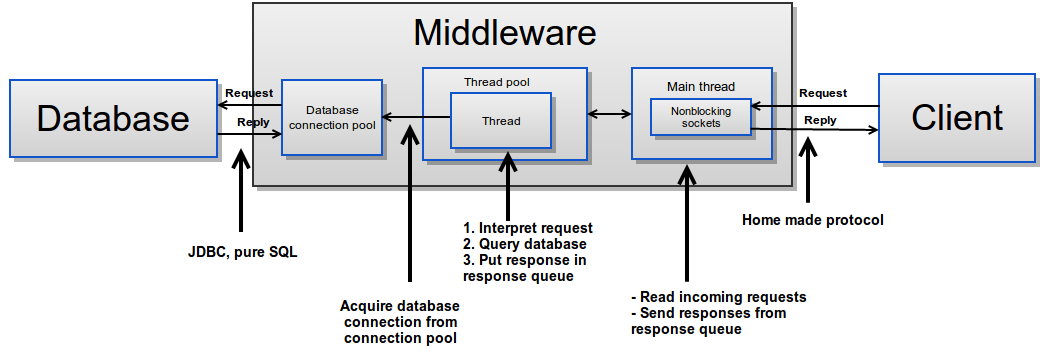
\includegraphics[scale=0.50]{implementation_high_level}}
             \caption{Graphical representation of implementation}
             \label{fig:implementation_high_level}
         \end{figure}
         \begin{enumerate}
             \item Client X sends request to middleware
             \item Middleware receives request on non-blocking socket in the network i/o
             \item Middleware passes raw request data on to worker thread X from the worker thread-pool
             \item Worker thread Y interprets the request
             \item Worker thread Y fetches a database connection from the database connection-pool, and performs a query matching the client's request
             \item Depending on the result of the query, worker thread Y figures out what to respond to the client and puts the response in the response queue
             \item Next time the network i/o thread goes through the response queue, it will find response Y and send it to client X
         \end{enumerate}
         
         There can, of course, be more than one middleware in our system. In this case the figure would be the same, as seen from the viewpoint of a client, because each client is connected to exactly one middleware.\\
        In the following subsections we explain our design decisions with regard to each component of our system: client, middleware, and database.

        \subsection{Client}
            As noted earlier, we have tried to keep the implementation of our client as simple as possible. This means that our client implementation only consists of code that implements the API described in Appendix \ref{sec:message_protocol_api}. Basically, our client code is a library that can be used in other Java applications to communicate with our middleware.\\
            \\
            The client has the following important Java \textbf{packages} and \textit{classes}:
            \begin{itemize}
                \item \textbf{asl}
                    \begin{itemize}
                        \item \textit{ThorBangMQ} - 'API': implements sendMessage, popMessage etc.
                        \item \textit{Message} - Representation of a message
                    \end{itemize}
                \item \textbf{asl.network}
                \begin{itemize}
                     \item \textit{SocketTransport} - Transport layer using sockets
                 \end{itemize} 
                \item \textbf{asl.infrastructure}
                 \begin{itemize}
                    \item \textit{MemoryLogger} - Logs to memory with the possibility to dump logs to a file later
                \end{itemize}
                \item \textbf{asl.infrastructure.exceptions}
                \begin{itemize}
                    \item \textit{InvalidClientException} - Invalid client id
                    \item \textit{InvalidQueueException} - Invalid queue id
                    \item \textit{InvalidMessageException} - Invalid message id
                    \item \textit{ServerException} - Unknown exception at server, something is very wrong
                \end{itemize}
            \end{itemize}

        \subsection{Middleware}
            \label{sec:description_middleware}
            In our middleware we have chosen to use non-blocking sockets instead of blocking sockets since it as a few properties that we like, one of which is that we don't have to spawn a new thread for every client that connects. This means that it has a very small impact on our server when a client connects, and that we can support many more clients simultaneously since the amount of threads in our program doesn't have to be linear to the amount of clients currently connected. There is an obvious disadvantage to choosing non-blocking sockets over blocking sockets though, which is that it can be harder to think about, implement, and work with.\\
            \\
            In an attempt to make our implementation simpler we decided to perform all network i/o in one thread of our program. Since we want to be able to handle multiple requests simultaneously, we pass data from the network i/o-thread to worker threads for interpretation and handling. These worker threads interpret incoming data and perform the database queries needed to handle requests. Responses to these requests are put in a response queue, which the network i/o-thread will empty as often as it can, by sending sending replies directly to clients.\\
            \\
            By moving interpretation and handling of requests to a thread different from the network i/o-thread, we have a place to perform our (blocking) calls to the database without blocking incoming requests. This is not entirely true though, since if there are more simultaneous requests than there are worker threads, the incoming request will be placed in a the thread pool queue and will effectively be blocked, though not it is not technically blocking the flow of the program.\\
            \\
            We have chosen to use a thread-pool for our worker threads in order to avoid the overhead of creating and deleting threads all of the time, and at the same time bound the  number of worker threads our program will spawn. This should make our system able to handle many requests than we have threads, at the cost of slower response times. It is important to note that this also means that the amount of simultaneous requests that our implementation can handle is equal to the minimum of the number of worker threads and the number of database connections given that no requests are invalid requests or HELLO requests (see A.1) since all but those go to the database. This is the case since a worker thread always needs a database connection to do its work (unless it received a malformed request, which shouldn't happen during our tests).\\
            \\
            With regard to database connections, we have chosen to use a connection-pool to avoid the overhead of setting up a new connection to the database each time we want to perform a query.\\
            \\
            The middleware consists of the following important Java \textbf{packages} and \textit{classes}:
            \begin{itemize}
                \item \textbf{asl}
                \begin{itemize}
                    \item \textit{Main} - Entry point of the program
                    \item \textit{IntervalLogger} - Logs test data every x second, configurable
                    \item \textit{GlobalCounters} - Holds global counters used during tests
                    \item \textit{Message} - Representation of a message
                    \item \textit{ServerSettings} - Configurable parameters of the server
                \end{itemize}
                \item \textbf{asl.infrastructure}
                \begin{itemize}
                    \item \textit{MemoryLogger} - Logs to memory with the possibility to dump logs to a file later
                \end{itemize}
                \item \textbf{asl.infrastructure.exceptions}
                \begin{itemize}
                    \item \textit{InvalidClientException} - Invalid client id
                    \item \textit{InvalidQueueException} - Invalid queue id
                    \item \textit{InvalidMessageException} - Invalid message id
                    \item \textit{ServerException} - Unknown exception at server, something is very wrong
                \end{itemize}
                \item \textbf{asl.network}
                \begin{itemize}
                    \item \textit{SocketTransport} - Transport layer using sockets
                \end{itemize}
                \item \textbf{asl.persistence}
                \begin{itemize}
                    \item \textit{PostgresPersistence} - Use Postgres as storage
                    \item \textit{InMemoryPersistence} - Use local memory as storage
                    \item \textit{LyingPersistence} - Don't store anything
                \end{itemize}
            \end{itemize}
            ~\\
            It should be noted that in our implementation of \textit{Pop message} we are using 'Peek message'. This causes two accesses to the database whenever a client performs a \textit{Pop message}-request that returns a message. We only realized this after doing our tests, which is why we kept the implementation as described.\\

            The flow of an individual request can be seen in Figure \ref{fig:middleware_flow}. Some things to note about Figure \ref{fig:middleware_flow}:

            \begin{itemize}
                \item The last step in the ClientRequestWorker, \textit{Add To Response Queue}, does this by using the interface \textit{asl.network.ITransport} which is passed to the ClientRequestWorker by the Socket I/O component. The ITransport-inferface declares just one function \textit{void Send(String s)}. The production implementation of this interface, \textit{SocketTransport}, keeps a reference to the response-queue which is continuously polled by the non blocking socket I/O. This way the Client Request Worker and the underlying networking implementation is decoupled.

                \item The Socket I/O and Job Creation component does more in one iteration than just check the response and requests queues. It also accepts client connections though this was omitted in the figure for clarity.
            \end{itemize}

   \begin{figure}[H]
                \centering
                \centerline{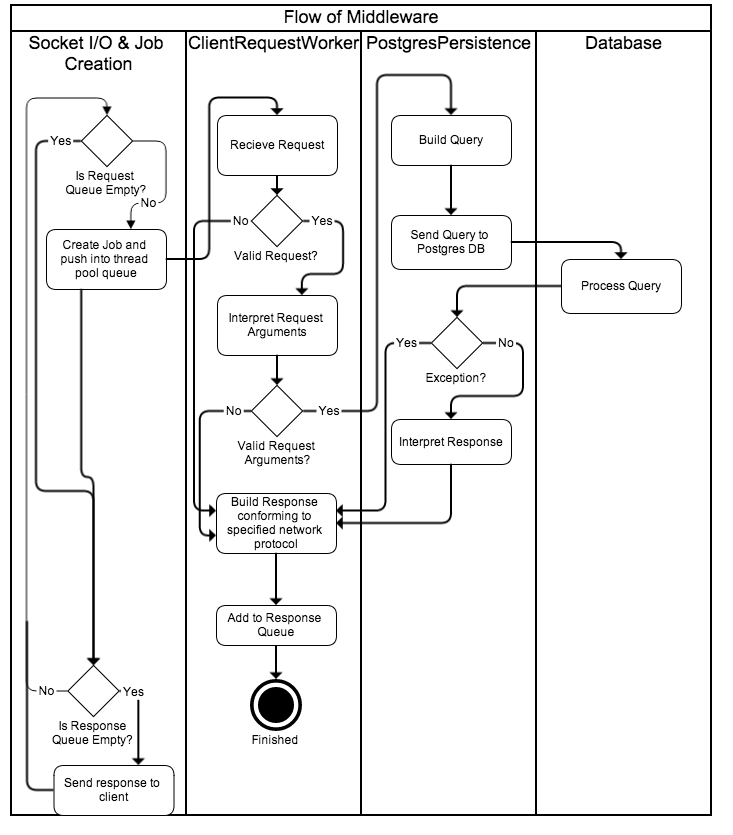
\includegraphics[scale=0.50]{middleware_flow}}
                \caption{The flow of the middleware's non-blocking sockets I/O and the path of an individual request.}
                \label{fig:middleware_flow}
            \end{figure}
        \subsection{Database}
            We have chosen to use a simple database schema with three tables: messages, queues, and clients. This schema is illustrated on Figure \ref{fig:database_schema}. We have used the following two multicolumn-indexes on the \textit{messages}-table: \textit{(receiver\_id, queue\_id, time\_of\_arrival)},\textit{(receiver\_id, queue\_id, priority)},\textit{(receiver\_id, queue\_id, priority)} and \textit{(receiver\_id, queue\_id, priority)}. 
            \begin{figure}[H]
                \centering
                \centerline{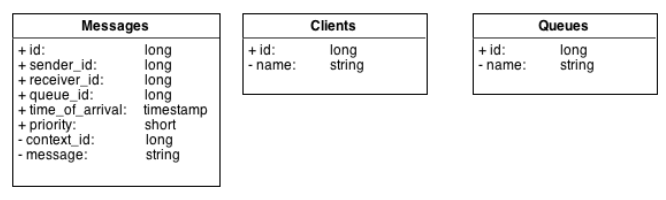
\includegraphics[scale=0.50]{database_schema}}
                \caption{Database schema}
                \label{fig:database_schema}
            \end{figure}
            ~\\
            When clients send messages to multiple queues at once, we have chosen to replicate messages in queues rather than having a many-to-many relationship in the database. This decision could affect performance since we're inserting more messages than we would, had we chosen to use a many-to-many relationship.\\
            \\
            Communication between the middleware and our database is done using JDBC, and we make SQL queries directly from our Java code. We decided not to use stored procedures, even though it requires slightly less data to represent each query, because we found it easier to implement and debug SQL directly in our Java code.

        \subsection{Communication protocol and API}
            We have chosen to use a very simple messaging protocol between the clients and the middleware. It uses an end of message token to differentiate messages from each other as we found it simpler to implement, compared to defining packets with headers containing message length and so on. We decided that our end of message token should be null, i.e. "\textbackslash0". All messages should be encoded in UTF8.\\
            Interpretation of requests and responses using our protocol is implemented in both server and client, in the SocketTransport classes. The full description of the communication protocol and API can be found in Appendix \ref{sec:message_protocol_api}.

    \section{Testing infrastructure}
        Our testing infrastructure is written in Python and does the following:
        \begin{itemize}
            \item Starts and stops servers
            \item Starts and stops experiments
            \item Fetches logs
            \item Generates graphs
        \end{itemize}
        ~\\
        Figure \ref{fig:testing_infrastructure} gives a graphical interpretation of our testing infrastructure.\\
         \begin{figure}[H]
             \centering
             \centerline{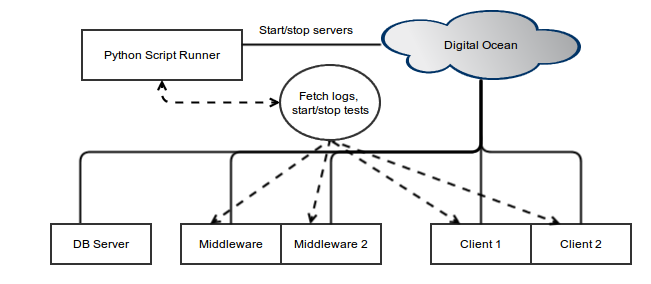
\includegraphics[scale=0.50]{testing_infrastructure}}
             \caption{Graphical representation of our testing infrastructure}
             \label{fig:testing_infrastructure}
         \end{figure}
        The infrastructure consists of 4 files:
        \begin{description}
            \item[main.py] Interface to start tests, see servers currently running etc.
            \item[infrastructure.py] Functions doing the actual infrastructure work.
            \item[droplets.py] Functions to start and stop servers (specific to DigitalOcean cloud provider).
            \item[gnuplot.py] Plots data.
        \end{description}
        ~\\
        Tests are defined by creating a folder in the test-definitions directory and creating three files: \textit{conf.txt}, which defines the configuration of a server, \textit{test.txt}, which defines the configuration of the clients and the number of servers and clients the test should be deployed on, and \textit{gnuplot.sh} which generates gnuplots when called with a test-result file as an argument.\\
        \\
        Other than the files described above, our testing infrastructure relies on the following python libraries: 
        \begin{description}
            \item[python-digitalocean] which can be installed via pip or found at \textit{https://pypi.python.org/pypi/python-digitalocean}.
            \item[psycopg2] which can be found at \textit{https://pypi.python.org/pypi/psycopg2}.
        \end{description}
        ~\\
        It should be noted that our testing infrastructure is very simple in that, for instance, it doesn't check for errors while running; it just assumes that everything executes successfully and continues on, even though that is not the case. We found this to be a somewhat of a mistake since it has caused us quite a bit of trouble during our testing.

    \section{Test definitions}
        \label{sec:test_definitions}
        This section contains a description of the tests that we performed during our measurements of our system. These tests can be configured in various ways in order to test different properties of our system.

        \subsection{Send and Pop Same Client}
            In this test all client threads continuously send 'SendMessage' and 'PopMessage' requests to the server (described in Appendix \ref{sec:message_protocol_api}). Each client thread sends a message to itself, then pops the message it just sent, and then repeats. This test is designed to keep the amount of messages in the database stable, while potentially putting a lot of load on the database - depending on the configuration of the parameters of the test. The test is configurable in: the number of (identical) threads to be spawned, time the test should run, the size of messages sent, the number of queues being used, and the amount of time each thread should sleep between sending requests. In all tests where nothing else is mentioned, the waiting time between requests is 0.\\
            \\
            \\
            Tests of this type perform the same amount of 'SendMessage' and 'PopMessage' requests, which means that the amount of messages in the system is kept stable. We expect that this test could put a lot of load on the server, especially if the amount of sleep-time is very low.

        \subsection{Standard test}
            \label{sec:standard_test}
            This test is an implementation of the test described in the project description, which we're supposed to be using for the traces. Our interpretation of the description, and our implementation, is as follows: A number of one-way clients bounce a single message randomly between each other, incrementing a counter in the message. Each one-way client keeps performing \textit{Pop message}-requests, checking if he got the message. A number of two-way clients each have a partner assigned, with whom they keep sending messages back and forth. Each two-way client keeps sending \textit{Pop message}-requests until he receives a message from his partner, and then sends a reply back. From this description we should note that the amount of \textit{Send Message}-requests doesn't change when the number of one-way clients increases, but it does when the number of two-way clients increases. Also to be noted, the number of \textit{Pop message}-requests increases when incrementing either of the two types of clients.\\
            \\
            The test is configurable in the amount of one-way clients and two-way clients it should use. Only too late to fix it did we realize that it would have been nice to be able to configure the size of messages sent, and the number of queues the messages are distributed over.\\
            \\
            Tests of this type perform many more 'PopMessage' requests than 'SendMessage' requests, but most of these 'PopMessage' requests will not actually find a message to pop, causing the total number of messages in the system to be kept stable.

        \subsection{Push peek pop}
            In this test a single client performs a configurable amount of a single type of request. This test is used for micro benchmarking each type of request.
            The test can be configured in: the type of requests sent and the amount of requests sent. This test can't be configured from the command line, and must be performed manually.\\
            \\
            Depending on the request being benchmarked, the amount of messages in the database may change over time. \textit{Send Message} requests, for instance, will increase the amount of messages in the system, while \textit{Pop message} will decrease the amount of messages in the system.

        \subsection{Timing measurements on the middleware}
            On the middleware we perform some timing measurements, measuring how much time is spent in different parts of our system. These names that we use for these parts are:\\
            \\
            \indent \textbf{IPersistence} which uses JDBC to query our database. Time spent in this class includes: think time for a database query and network delays from our middleware to the database and back again.\\
            \\
            \indent \textbf{Client Request Worker} which interprets user requests. Time spent in this class includes: string manipulation to interpret user requests, calling of methods in IPersistence, creating a response for the client and putting it in the response queue. The time spent in IPersistence is subtracted from the time measured in this class such that time measured for this class doesn't include the time it takes to perform calls in IPersistence.\\
            \\
            \indent \textbf{Socket I/O \& Queuing} which handles communication with clients. Time spent in this class includes: reading from and writing to a client socket, handing data read from client sockets to a worker thread, and the time requests spend waiting to get handed to a worker thread.
            \\
            \\
            Figure \ref{fig:timing_measurements} is a graphical representation of these measurements points.\\
            \begin{figure}[H]
                \centering
                \centerline{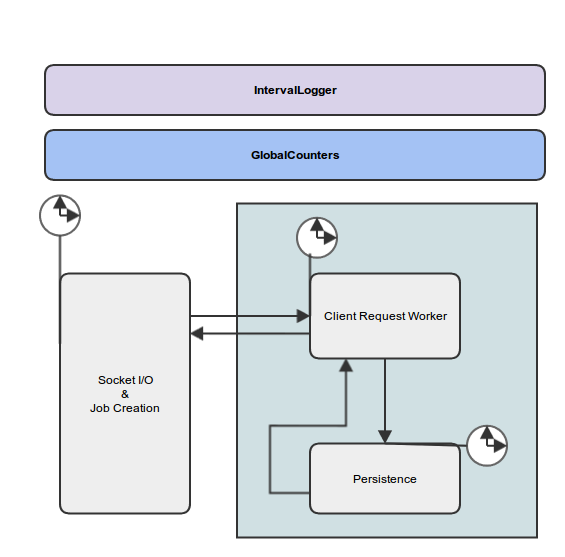
\includegraphics[scale=0.50]{timing_measurements}}
                \caption{Graphical representation of timing measurements done on middleware}
                \label{fig:timing_measurements}
            \end{figure}

    \section{Tests and results}
        \label{sec:tests_and_results}
        In this section we describe the tests we have performed, present the results and give a short commentary on what can be seen on the graphs. We interpret and analyze these results in Section \ref{sec:analysis}.\\
        \\
        In our tests we have focused on peeking, popping, and sending messages. We decided to have this focus because we work under the assumption that these types of requests are vastly more frequent than all other types of requests (create queue, remove queue etc.), and that the performance of the system as a whole will be dominated by these three types of requests.\\
        \\
        We have performed our tests using machines from the cloud hosting provider DigitalOcean.com, from whom we got a 200\$ coupon to run experiments. Running our tests on a cloud host has some obvious downsides w.r.t. the results of our tests, since we can't know for sure which hardware our tests are run on, and if we are sharing this hardware with anyone.\\
        We have run all of our experiments on machines with: 4GB memory, SSD storage, and 2 logical CPU cores. Due to the way DigitalOcean provide their servers, we can't really tell how much computing power these logical CPUs provide, or whether there are any neighbors on the hardware. In order to compensate for this we've run all of our experiments for at least 10 minutes each, to see whether the observed performance is somewhat consistent.\\
        \\
        For all tests where nothing else is mentioned, the amount of messages in the database has been kept steady at around 20,000 messages, and the size of messages (payload of a \textit{Send message} request) is very low (around 5 bytes)\\
        \\
        It is important to note that all of the following tests use blocking sockets (on the client side) to send requests. This means that each of our clients can not have more than one ongoing request or, put a different way, the total number of simultaneous requests in the system is at most the number of clients. In the literature this is referred to as a closed system.\\
        \\
        In order to try to explain the performance of our system, we have identified the following parameters that we wish to test.
        \begin{itemize}
            \item Client
            \begin{itemize}
                \item Size of messages
                \item Frequency of requests
                \item Total number of clients
                \item Type of Requests
            \end{itemize}
            \item Middleware
            \begin{itemize}
                \item Number of middleware instances
                \item Number of database connections
                \item Number of worker threads
                \item Impact of using database vs. not storing messages at all
            \end{itemize}
            \item Database
            \begin{itemize}
                \item Size of dataset
                \item Number of queues which messages are distributed over
            \end{itemize}
        \end{itemize}

        \subsection{Code profiling}
            In order to figure out exactly where our code spends the most time and to confirm that out measurements were valid, we've used the code profiling tool VisualVM (\textit{http://visualvm.java.net/}). We have performed code profiling during multiple different tests with multiple different configurations. Every time we ran the profiler we got almost identical results. The profiling runs shown on Figure \ref{fig:code_profiling_send_pop_same_client} and \ref{fig:code_profiling_standard_test} were run for approx. 3 minutes with 80 clients sending very small messages (around 5 bytes). These two tests show the general results we got with all configurations of these two types of tests. Our code spends almost all of the time, as shown on Figure \ref{fig:code_profiling_send_pop_same_client} and \ref{fig:code_profiling_standard_test}, communicating with and waiting for the database. In fact, the top 3 most time consuming tasks are all due to communication with the database. If we put the time consumption of these tasks together, they add up to 83.1\% for 'Send and Pop Same Client' and 87.5\% for 'standard test'.
            In order to figure out exactly where our code spends the most time, we've used the code profiling tool VisualVM (\textit{http://visualvm.java.net/}). We have performed code profiling during multiple different tests with multiple different configurations. Every time we ran the profiler we got almost identical results. The profiling runs shown on Figure \ref{fig:code_profiling_send_pop_same_client} and \ref{fig:code_profiling_standard_test} were run for approx. 3 minutes with 80 clients sending very small messages (around 5 bytes). These two tests show the general results we got with all configurations of these two types of tests. Our code spends almost all of the time, as shown on Figure \ref{fig:code_profiling_send_pop_same_client} and \ref{fig:code_profiling_standard_test}, communicating with and waiting for the database. In fact, the top 3 most time consuming tasks are all due to communication with the database. If we put the time consumption of these tasks together, they add up to 83.1\% for \textit{Send and Pop Same Client} and 87.5\% for \textit{Standard test}.
            \begin{figure}[H]
                \hspace{-1.5cm}
                \centerline{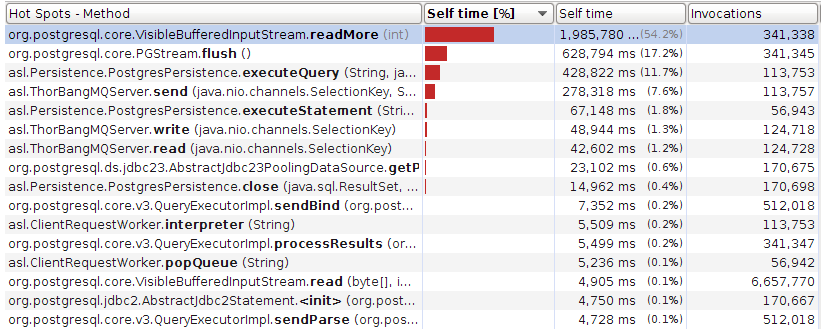
\includegraphics[scale=0.50]{code_profiling_send_pop_same_client}}
                \caption{3 minutes of profiling during \textit{Send and Pop Same Client} with 80 clients, very small messages}
                \label{fig:code_profiling_send_pop_same_client}
            \end{figure}
            \begin{figure}[H]
                \hspace{-1.5cm}
                \centerline{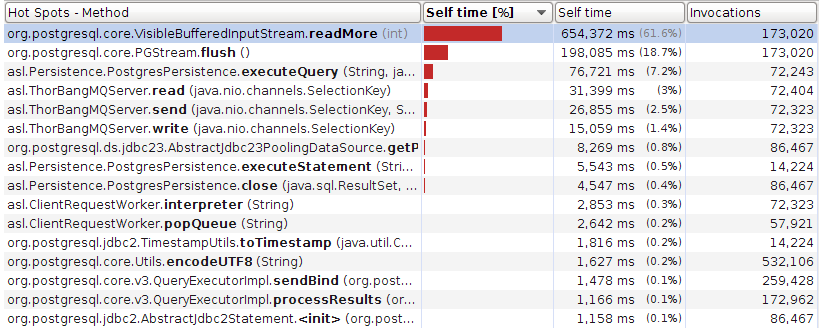
\includegraphics[scale=0.50]{code_profiling_standard_test}}
                \caption{3 minutes of profiling during \textit{Standard test} with 80 clients, very small messages}
                \label{fig:code_profiling_standard_test}
            \end{figure}
            ~\\
            On both Figures we also see that \textit{ThorBangMQServer.read} and \textit{ThorBangMQServer.send} take up a lot of time: 8.8\% for \textit{Send and Pop Same Client} and 5.5\% for \textit{Standard test}. These two calls are responsible for communication with clients, where 'read' gets clients' requests and 'send' sends replies to clients.\\
            On both Figures we also see that \textit{ThorBangMQServer.read} and \textit{ThorBangMQServer.send} takes up some time: 8.8\% for 'Send and Pop Same Client' and 5.5\% for 'Standard test'. These two calls are responsible for communication with clients, where 'read' gets clients' requests and 'send' sends replies to clients.\\
            \\
            The last thing we note is that 'ThorBangMQServer.write' takes up 1.3\% and 1.4\% of \textit{Send and Pop Same Client} and \textit{Standard test} respectively. This method is responsible for putting responses into the response queue (as explained in Section \ref{sec:description_middleware}) and is performed by worker threads when they are done handling a client's request.

            % Bottlenecks
            % Most expensive operations that determine the overall performance

        \subsection{Long trace}
            The figures in this section show the overall stability of the system while under moderate to high system load for 4 hours. The following test are of the type \textit{Standard test}. In this test we expect to see that the system behaves in a somewhat stable manner meaning that we have a low standard deviation of our measurements. We expect that the system will have queued jobs at all times and that the throughput will be stable and that the response times may vary since we are doing different types of calls: \textit{Send Message} and \textit{Pop Message}. Clients and worker-threads and database connections increases since, as described in Section \ref{sec:description_middleware}, the number of database connections and worker-threads bounds the amount of requests that will be handled simultaneously by our middleware. We don't think that this will keep scaling though, since increasing the number of database connections gives the opportunity to put more load on the database which, at some point, will not be able to cope with the increased load.\\
            \\
            The following figure have been plotted with the throughput of reads and writes individually, and have more reads than writes in the system for the reasons described in Section \ref{sec:standard_test}.\\
            \\
            On the longest running trace we have, running a total of 4 hours, we had a total of 300 clients and 50 worker threads and database connections in the middleware. The results of this test is shown on Figure \ref{fig:4h_throughput_respTime}. Here we see that the system behaves in a very stable manner throughout the test.

            \begin{figure}[H]
                \centering
                \centerline{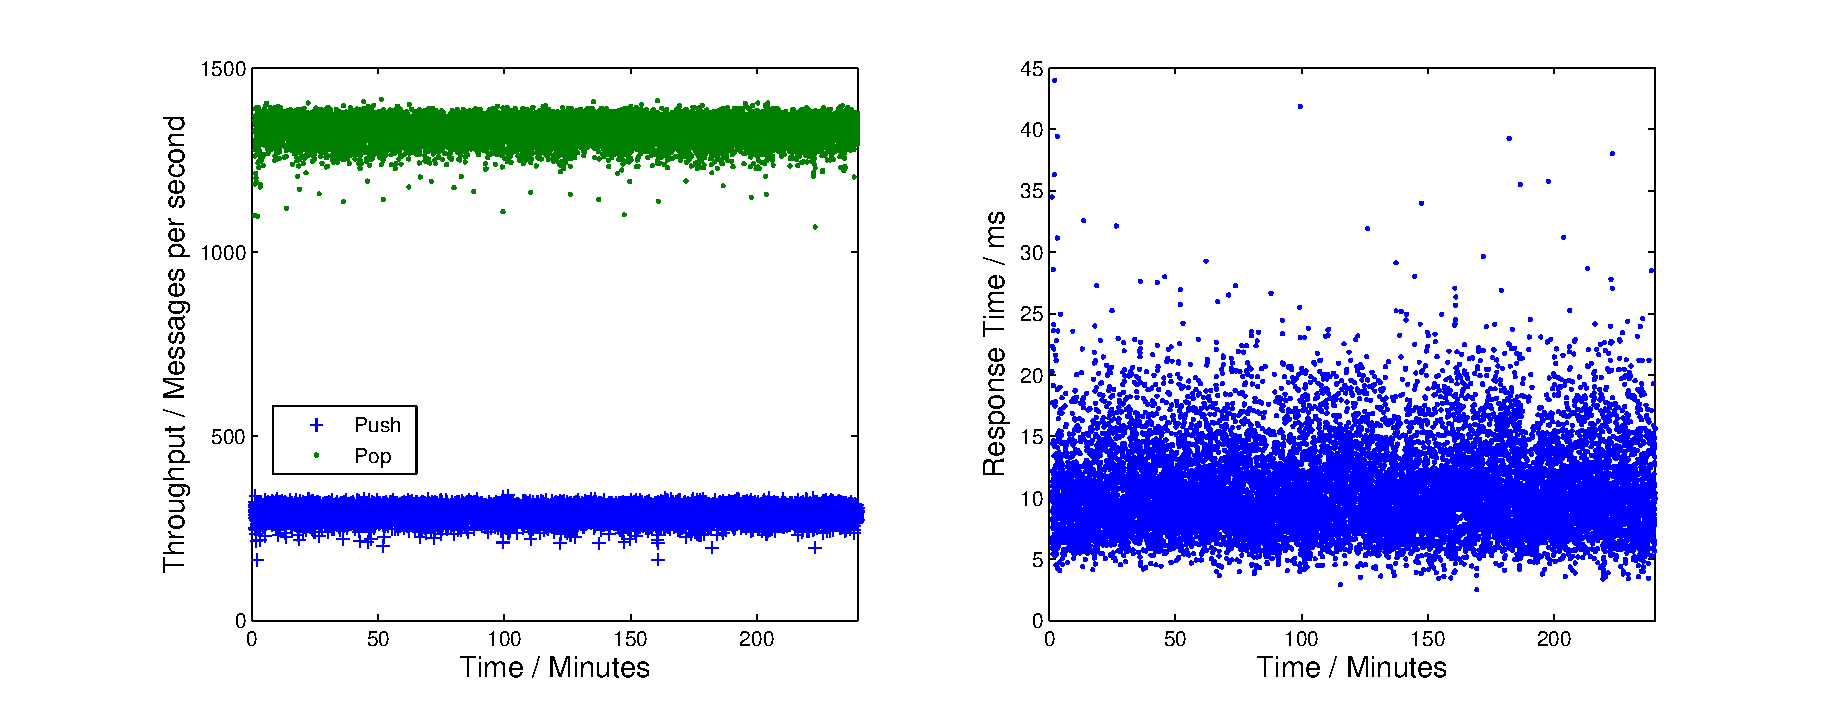
\includegraphics[scale=0.5]{4h_throughput_respTime}}
                \caption{The throughput of the system while under load from the \textit{Standard Test} with 200 one-way clients and 100 two-way clients. Using 1 middleware with 50 worker threads and 50 database connections. The dotted red line shows the average throughput and the solid lines the standard deviation.}
                \label{fig:4h_throughput_respTime}
            \end{figure}
            ~\\
            ~\\
            Table \ref{table:throughput_4h_test} and Table \ref{table:thinktimes_4h_test_components} show the results from our long trace in numbers. We see that the confidence intervals are low, which means that the system behaves very stable. This is also evident when we look at Figure \ref{fig:4h_throughput_respTime}.\\

            \begin{table}[H]
                \centering
                \begin{tabular}{|c|c|}
                   \hline 
                    \textbf{Request Type} & \textbf{Mean Throughpout} (Requests per second) \\ 
                        \hline 
                        Send/Push Message& $293.91 \pm [-28.91 , 21.09]$\\ 
                        \hline 
                        Pop Message & $1331.73 \pm [-53.73 , 42.27]$ \\ 
                        \hline 
                        Total & $1625.63 \pm [-77.48 , 59.37]$\\ 
                        \hline 
                    \end{tabular}
                    \caption{Breakdown of the think times in the system while under load from \textit{Standard Test} with 200 one-way clients and 100 two-way clients. Using 1 middleware with 50 worker threads and 50 database connections.}
                    \label{table:throughput_4h_test}
                \end{table} 


            \begin{table}[H]
                \centering
                \begin{tabular}{|c|c|}
                   \hline 
                    \textbf{Component} & \textbf{Mean Think Time} (ms) \\ 
                        \hline 
                        Socket I/O \& Queuing & $1.11 \pm [-0.83 , 1.80]$\\ 
                        \hline 
                        CRW & $0.12 \pm [-0.10 , 0.11]$ \\ 
                        \hline 
                        IPersistence & $9.43 \pm [-3.89 , 5.52]$\\ 
                        \hline 
                        Total & $10.66 \pm [-4.54 , 7.06]$\\ 
                        \hline 
                    \end{tabular}
                    \caption{Breakdown of the think times in the system while under load from \textit{Standard Test} with 200 one-way clients and 100 two-way clients. Using 1 middleware with 50 worker threads and 50 database connections.}
                    \label{table:thinktimes_4h_test_components}
                \end{table} 
        The logs for this test can be found in the \textit{4h-trace} folder.


        \subsection{Micro benchmarks}
            The tests in this section are made to test the performance of single types of requests. The following tests have been performed on a single middleware with 50 worker threads and 50 database connections. The amount of worker threads and database connections should not matter to this test though, since we use only a single client which will only send the next request when it has received a reply to the previous (closed system). This claim is tested in Section \ref{sec:difference_in_dbcons_and_worker_threads}.

            \subsubsection{Send message}
                \label{sec:micro_send_message}
                In this test a single client continuously sends \textit{Send message} requests to the middleware. This means that the size of the dataset increases from 20,000 to 520,000 in the span of the test.\\
                \\
                On Figure \ref{fig:thinktime_500k_push} we see that the amount of time spent on each request is dominated by the time it takes to get a response from the database, shown by the scattered dots in the top of the graph. In Table \ref{table:thinktime_500k_push} the data for this graph is given, showing that the time spent in IPersistence is at least an order of magnitude higher than the rest of the system. We also see that the standard deviation of time spent in IPersistence is much higher than it is for the two other measurements.\\
                Figure \ref{fig:responsetime_500k_push} shows the response time throughout the 500,000 \textit{Send message} requests. On this graph we see that the response time is rather stable, except for the few scattered points in the top of the graph.

                \begin{figure}[H]
                \centering
                    \centerline{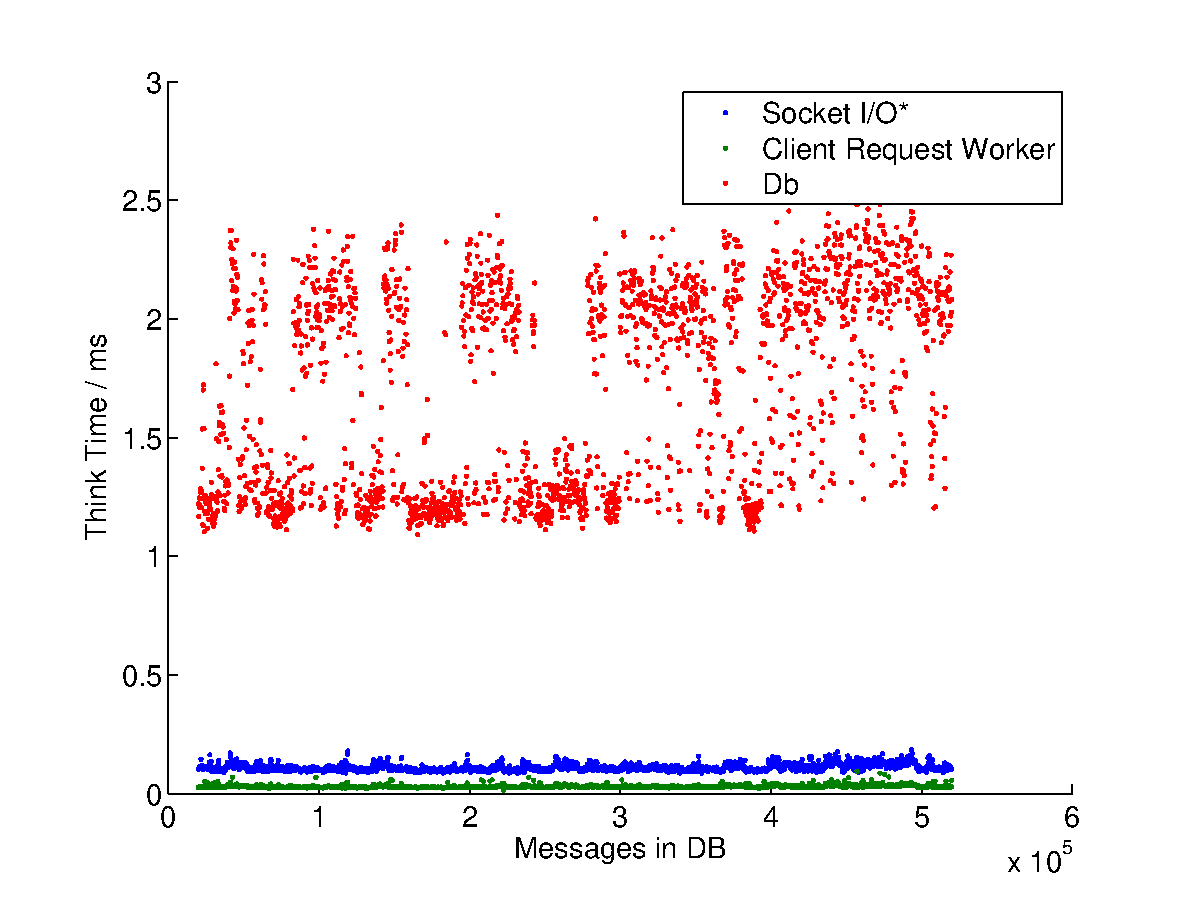
\includegraphics[scale=0.50]{thinktime_500k_push}}
                    \caption{The think time for send message request. Each data point represents an individual request. A total of 500,000 requests sent sequentially each after the other.}
                    \label{fig:thinktime_500k_push}
                \end{figure}
                \begin{table}[H]
                    \centering
                    \begin{tabular}{|c|c|c|}
                        \hline 
                        \textbf{Component} & \textbf{Average Think Time} (ms) & \textbf{Standard Deviation (ms)} \\ 
                        \hline 
                        Socket I/O \& Queuing & $0.111 \pm [-0.0163 , 0.0299]$ &0.0145\\ 
                        \hline 
                        CRW & $0.0310 \pm [-0.0052 , 0.0098]$ &0.0057\\ 
                        \hline 
                        IPersistence & $1.714 \pm [-0.5508 , 0.5903]$ &0.427\\ 
                        \hline 
                    \end{tabular}
                    \caption{Average think time, confidence interval, and standard deviation for 500,000 \textit{Send message} requests}
                    \label{table:thinktime_500k_push}
                \end{table} 
                
                \begin{figure}[H]
                    \centering
                    \centerline{\includegraphics[scale=0.50]{responsetime_500k_push}}
                    \caption{The response time for send message request. Each data point represents an individual request. A total of 500,000 requests sent sequentially each after the other.}
                    \label{fig:responsetime_500k_push}
                \end{figure}
                ~\\
                \\

        The logs for this test can be found in \textit{micro-benchmarks/sequential\_requests}.


        \subsection{Response Times for Requests}
                \begin{table}
                    \begin{tabular}{|c|c|}
                        \hline 
                        \textbf{Type of Request} & \textbf{Response Time} (ms) \\ 
                        \hline 
                        Pop & $3.997 \pm 0.021$ \\ 
                        \hline 
                        Peek & $2.022 \pm 0.038$ \\ 
                        \hline 
                        Push & $1.856 \pm 0.61294$ \\ 
                        \hline 
                    \end{tabular} 
                    \caption{The response times for the requests: \textit{Pop message}, \textit{Send message}, and \textit{Peek message}. Using 50 worker threads, 50 db connections, 1 client and 1 middleware.}
                    \label{tbl:response_times_requests}
                \end{table}

        The logs for this test can be found in \textit{micro-benchmarks/sequential\_requests}.

        \subsection{Breakdown of Think Times}
            \begin{figure}[H]
                    \centering
                    \centerline{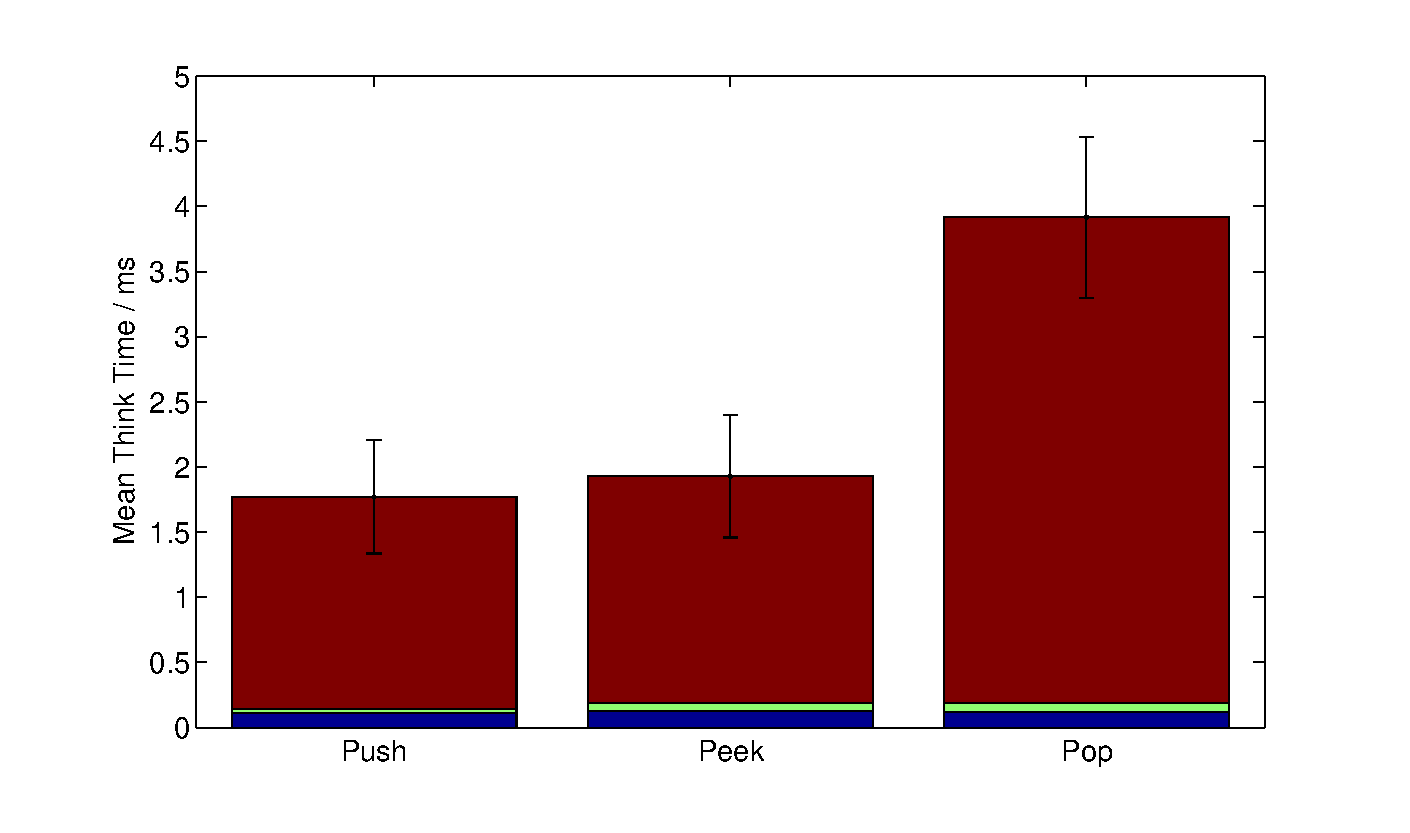
\includegraphics[scale=0.50]{thinktime_push_peek_pop}}
                    \caption{Breakdown of the thinktime for Send Message, Peek, and Pop requests. Using 1 client sending these requests sequentially to 1 middleware with only this client.}
                    \label{fig:thinktime_push_peek_pop}
             \end{figure}

        The logs for this test can be found in \textit{micro-benchmarks/sequential\_requests}.

            \subsubsection{Pop message}
                In this test a single client continuously sends a total of 500,000 \textit{Pop message} requests. This test was run after the \textit{Send message} test described in the last subsection, which means that there was a total of 520,000 messages in the database when this test was started. In this test the amount of messages in the database goes from 520,000 to 20,000.\\
                \\
                On Figure \ref{fig:thinktime_500k_pop} we see that the think time of the database (IPersistence) dominates the think time of the middleware. We also see that it has as specific pattern over time. We see that the think-time decreases and becomes more stable when the number of messages in the database decreases. On Table \ref{table:think_time_send_message} we see the numbers with 90\% confidence intervals.


                \begin{figure}[H]
                    \centering
                    \centerline{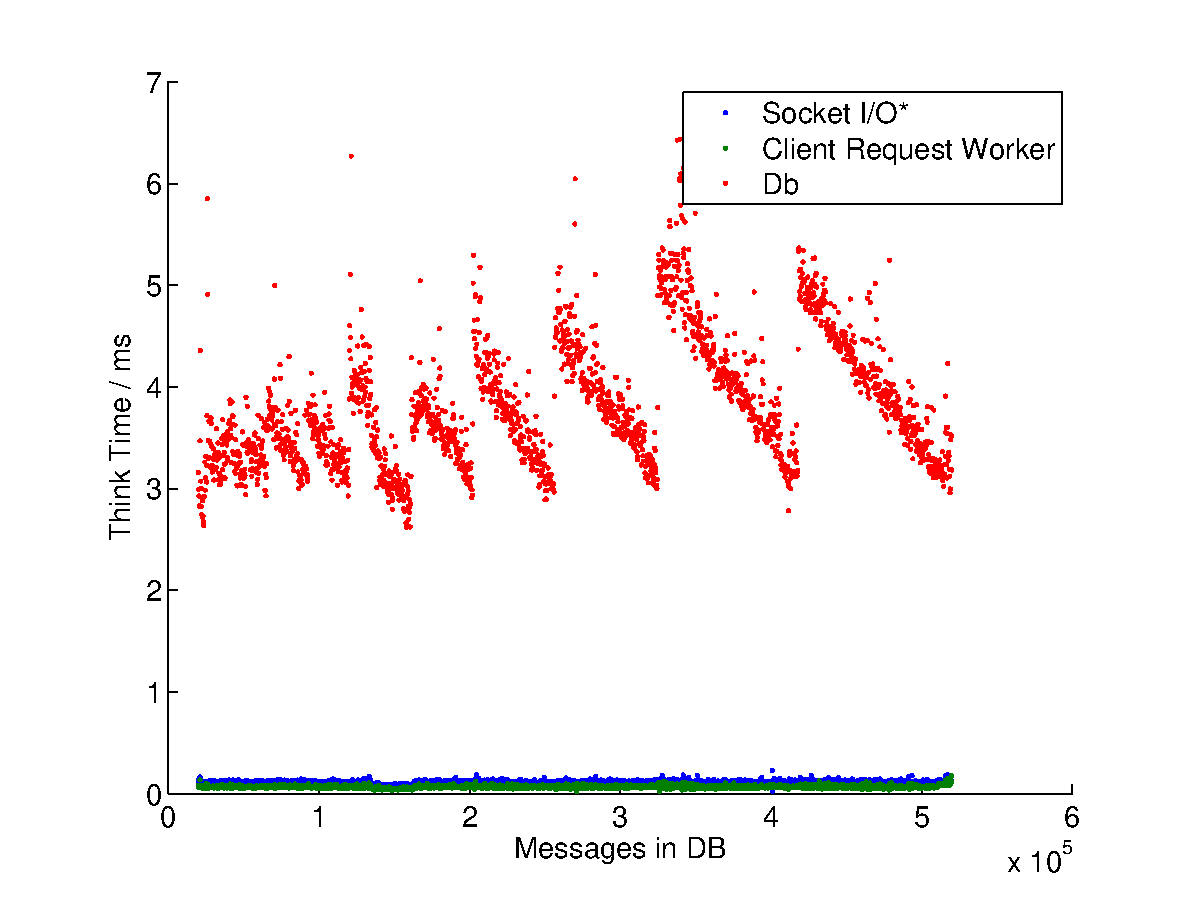
\includegraphics[scale=0.50]{thinktime_500k_pop}}
                    \caption{The think-time of the middleware during 500,000 \textit{Pop message} requests. Each data point represents an individual request.}
                    \label{fig:thinktime_500k_pop}
                \end{figure}

                \begin{table}[H]
                    \centering
                    \begin{tabular}{|c|c|c|}
                        \hline 
                        \textbf{Component} & \textbf{Mean Think Time} (ms)\\ 
                        \hline 
                        Socket I/O \& Queuing & $0.118\pm0.021$ \\ 
                        \hline 
                        CRW & $0.069\pm [-0.0192 , 0.0227]$ \\ 
                        \hline 
                        IPersistence & $3.810\pm1.164$ \\ 
                        \hline 
                    \end{tabular}
                    \caption{Think times of the three different components of our system which we measure.}
                    \label{table:think_time_send_message}
                \end{table}
                
                \begin{figure}[H]
                    \centering
                    \centerline{\includegraphics[scale=0.50]{responsetime_500k_pop}}
                    \caption{The response time for \textit{Pop message} request. Each data point represents an individual request. A total of 500,000 requests sent sequentially each after the other.}
                    \label{fig:responsetime_500k_pop}
                \end{figure}                
                ~\\
                \\           
                
        The logs for this test can be found in \textit{micro-benchmarks/sequential\_requests}.
            \subsubsection{Peek message}
                In this test a single client continuously sends \textit{Peek message}-requests to the middleware. The size of the dataset stays the same since \textit{Peek message} doesn't actually modify the dataset.\\
                \\
                On Figure \ref{fig:thinktime_500k_peek} we see that the response time of the database dominates the think-time of the middleware. We see that the response time of the database varies consistently between around 1.25 and 2.5.

                \begin{figure}[H]
                    \centering
                    \centerline{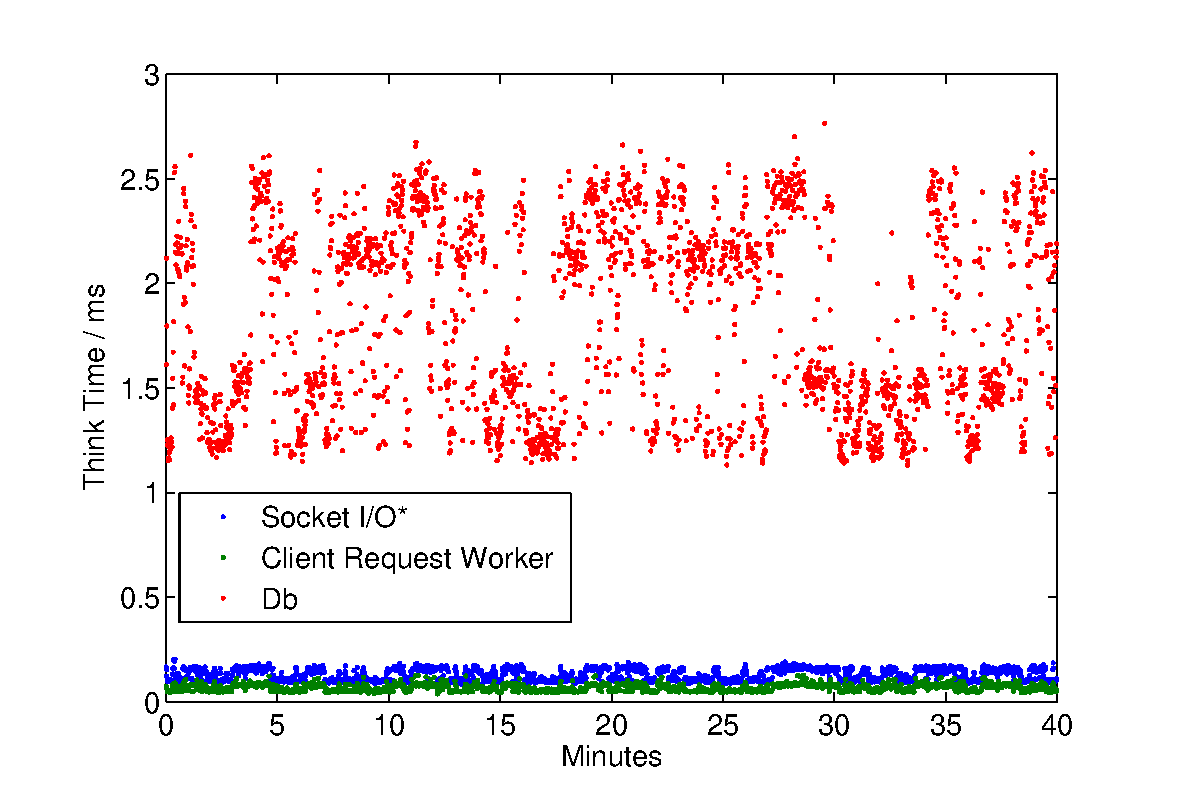
\includegraphics[scale=0.50]{thinktime_500k_peek}}
                    \caption{The think time in the server for \textit{Peek message} request. Each data point represents an individual request. A total of 500,000 requests sent sequentially each after the other.}
                    \label{fig:thinktime_500k_peek}
                \end{figure}

                \begin{figure}[H]
                    \centering
                    \centerline{\includegraphics[scale=0.50]{responsetime_500k_peek}}
                    \caption{The response time for \textit{Peek message} request. Each data point represents an individual request. A total of 500,000 requests sent sequentially each after the other.}
                    \label{fig:responsetime_500k_peek}
                \end{figure}
                
                \begin{table}[H]
                    \centering
                    \begin{tabular}{|c|c|c|}
                        \hline 
                        \textbf{Component} & \textbf{Mean Think Time} (ms)\\ 
                        \hline 
                        Socket I/O \& Queuing & $0.1292\pm [-0.0342 , 0.0381]$\\ 
                        \hline 
                        CRW & $0.0658\pm [-0.0194 , 0.0220]$\\ 
                        \hline 
                        IPersistence &$1.8264\pm [-0.6189 , 0.6532]$\\ 
                        \hline 
                    \end{tabular}
                    \caption{Average think time, confidence interval, and standard deviation for 500,000 \textit{Send message} requests}
                    \label{table:thinktime_500k_peek}
                \end{table} 
                ~\\
                \\
                The raw data from these tests can be found in the log-folder, in the subfolders
                \begin{itemize}
                    \item folders
                \end{itemize}

        The logs for this test can be found in \textit{micro-benchmarks/sequential\_requests}.

        \subsection{Difference in message size}
            \begin{figure}[H]
                    \centerline{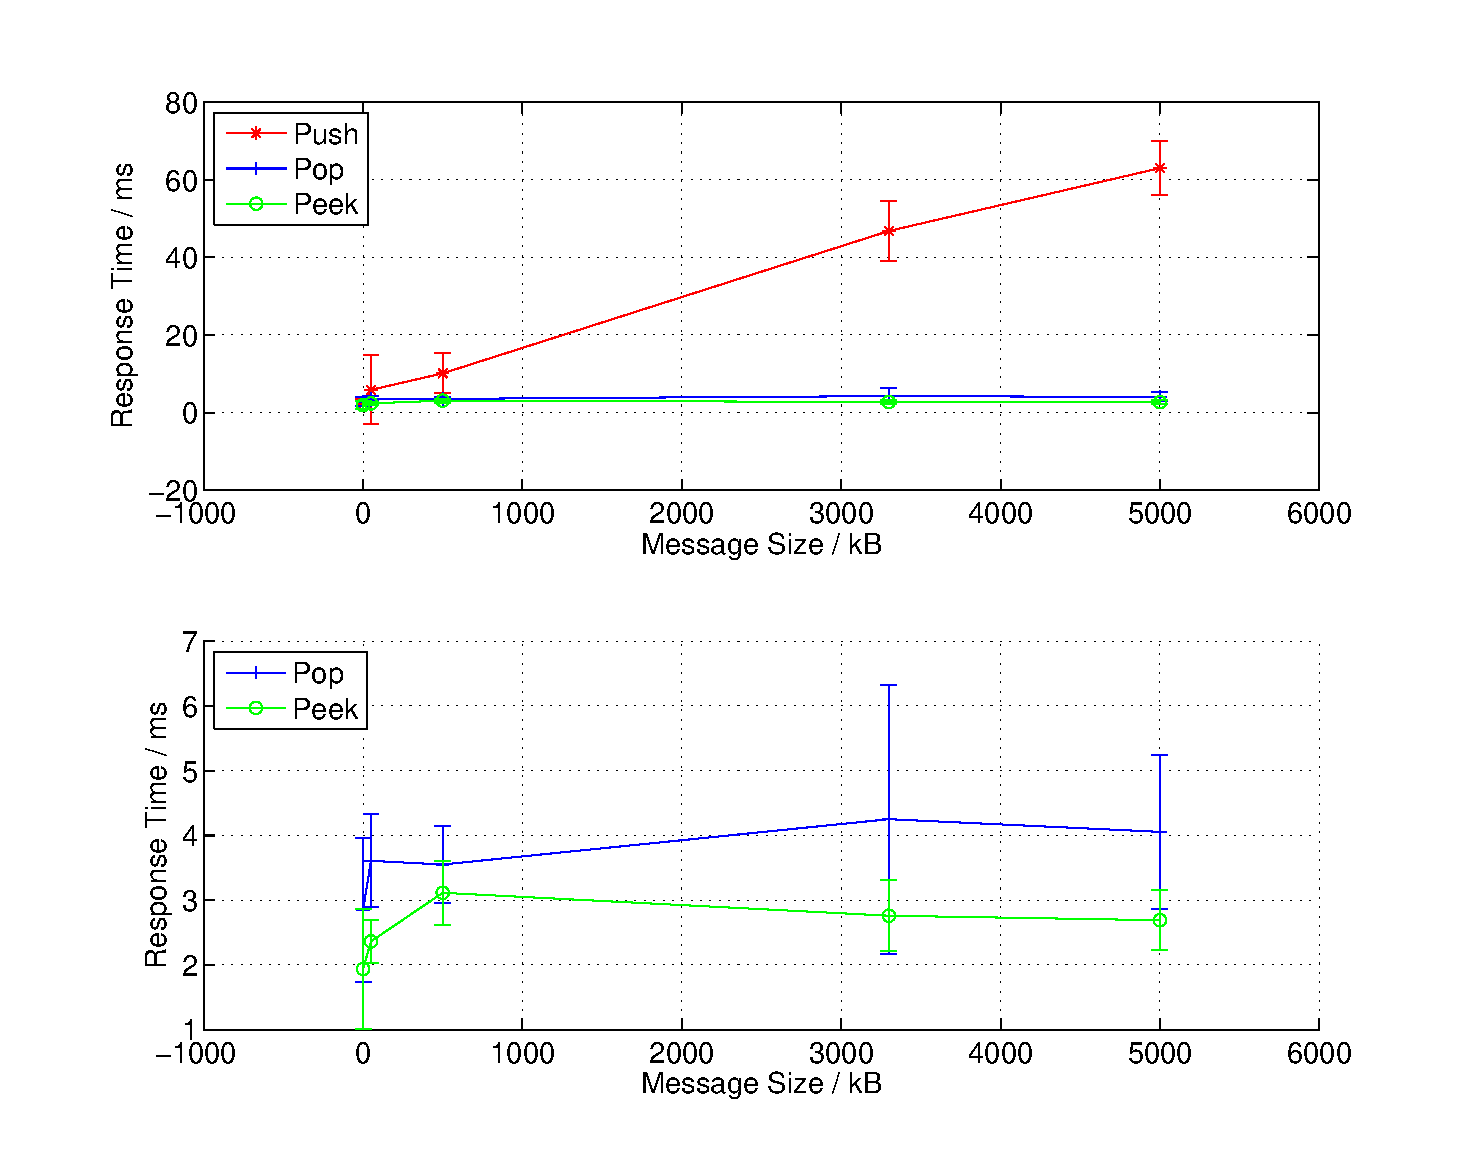
\includegraphics[scale=0.60]{responsetime_msgsize}}
                    \caption{The response time for \textit{send message}, \textit{Peek message}, and \textit{Pop message} as a function of the message size. The peeking and popping curves are also shown again in the lower graph without response time of \textit{Send message} for clarity.}
                    \label{fig:responsetime_msgsize}
                \end{figure}

        The logs for this test can be found in \textit{micro-benchmarks/message-content-size}.


        \subsection{Difference in size of dataset}
            \label{sec:difference_in_size_of_dataset}
            In this test we want to see what the difference of the size of the dataset matters to our system's performance. In this test we're using \textit{Send and Pop Same Client}, varying the number of messages initially stored in the database. From this test we expect that an increase in the size of the data set will increase the think-time of the database, resulting in a lower throughput.
            \begin{figure}[H]
                \centerline{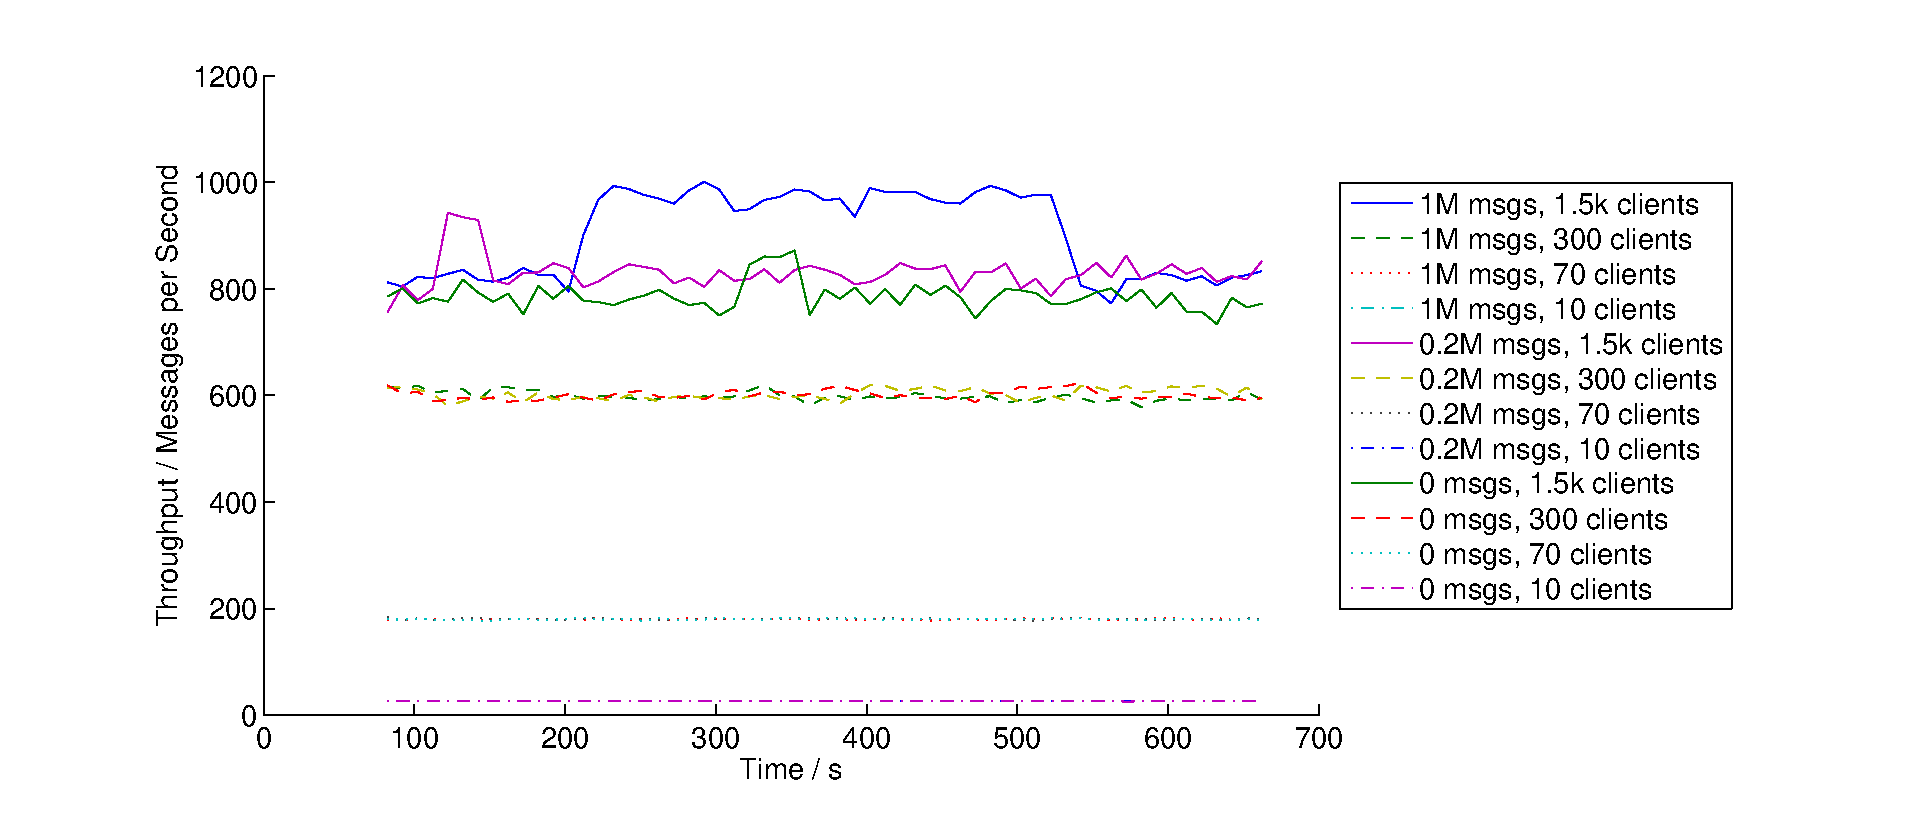
\includegraphics[scale=0.55]{msg_db_clients}}
                \caption{The throughput when running \textit{Standard Test} varying number of clients and number of messages stored in database prior to test start. Run on one middleware having 50 worker threads and 50 database connections.}
                \label{fig:msg_db_clients}
            \end{figure}
            ~\\
            \\
            The raw data from these tests can be found in the log-folder, in the subfolders
            \begin{itemize}
                \item \textit{sendandpopsameclient\_diff\_clients\_msgsize-10b}
                \item \textit{sendandpopsameclient\_diff\_clients\_msgsize-1mb}
                \item \textit{sendandpopsameclient\_diff\_clients\_msgsize-10mb}
            \end{itemize}


            \begin{figure}[H]
                \centerline{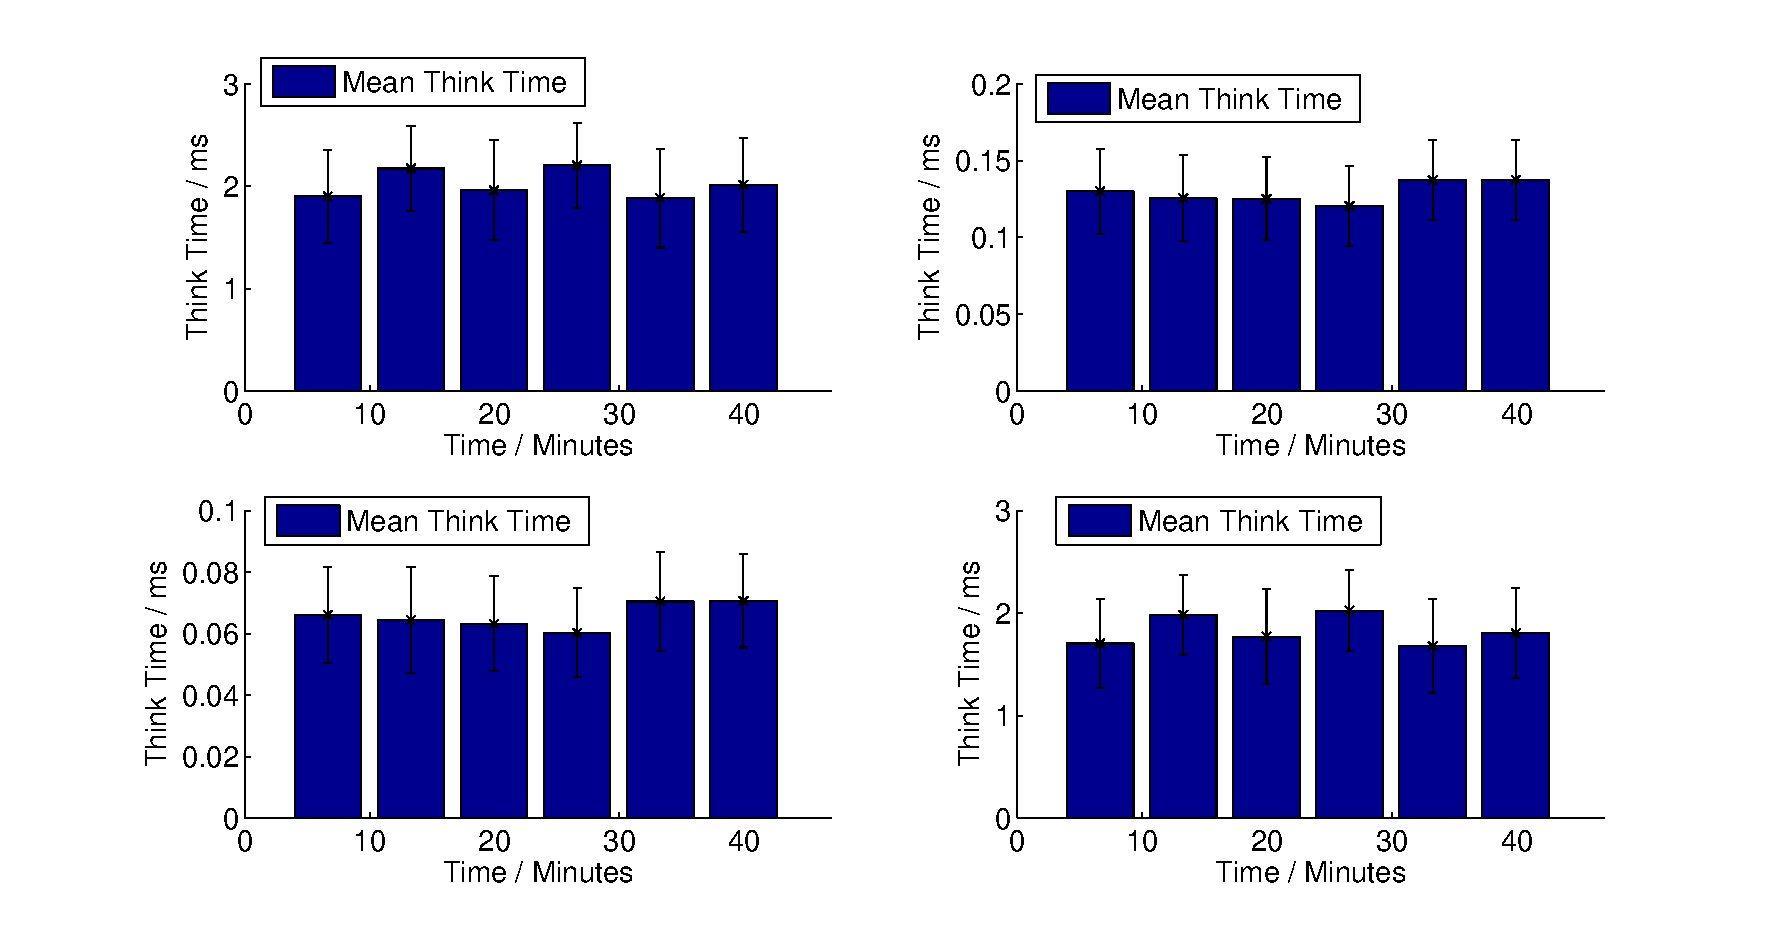
\includegraphics[scale=0.55]{resptime_as_function_of_msgs_in_db_peek}}
                \caption{The response time over time when performing sequential peek-requests using one (1) client and 520k messages in the database. The figure shows the total throughput (top left), think time in Socket I/O and job creation (top right), Client Request Worker (bottom left) and Persistence (bottom right)}
                \label{fig:resptime_as_function_of_msgs_in_db_peek}
            \end{figure}

            \begin{figure}[H]
                \centerline{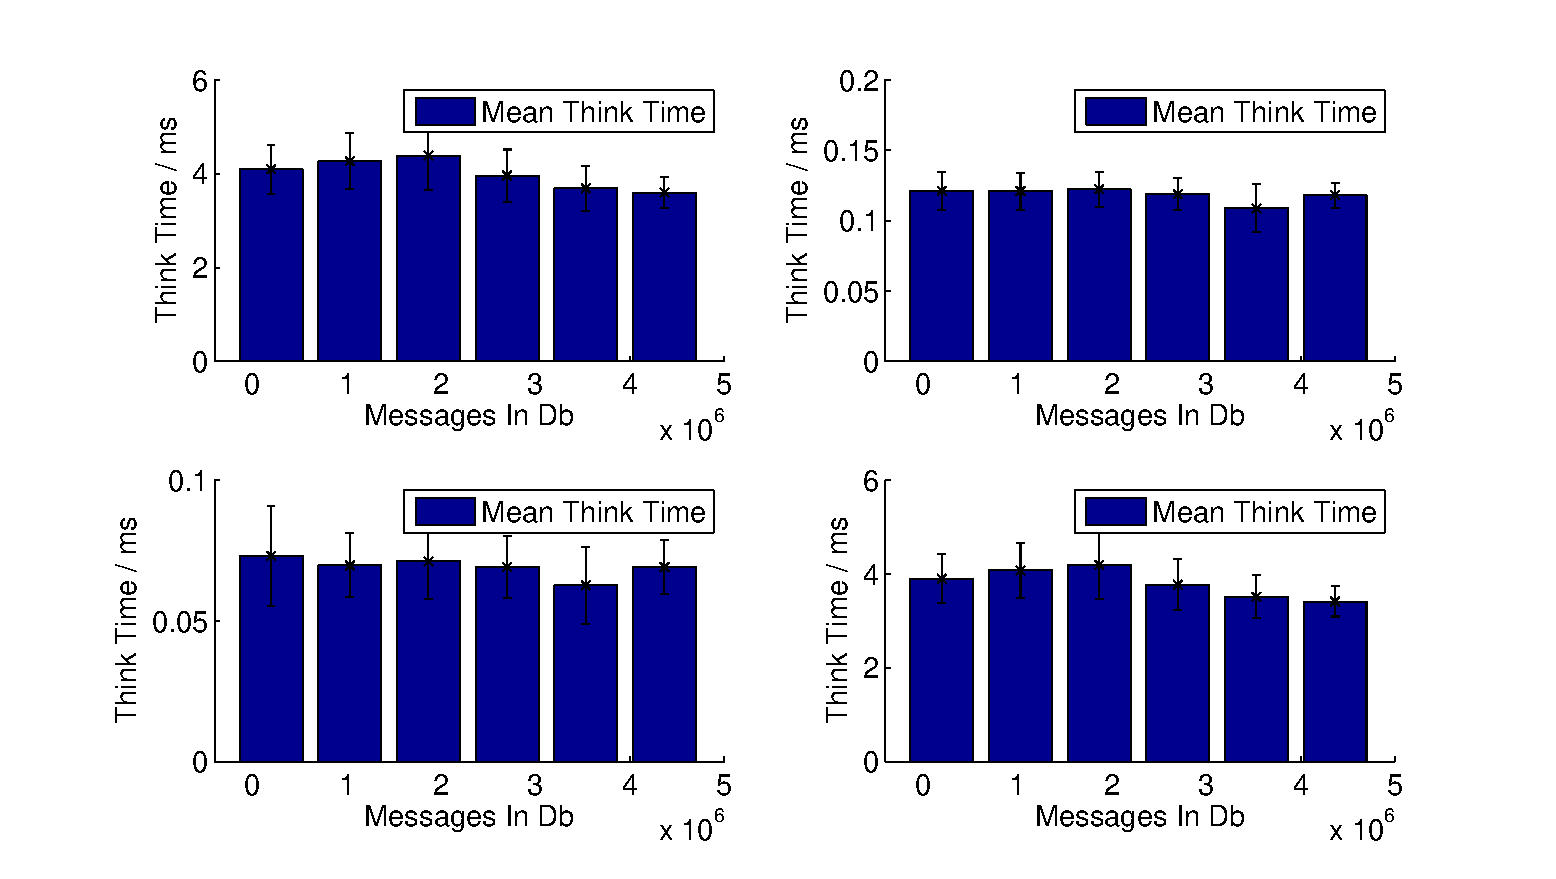
\includegraphics[scale=0.55]{resptime_as_function_of_msgs_in_db_pop}}
                \caption{The response time as a function of number of messages in the database when performing sequential pop-requests using one (1) client and initially 520k messages in the database. The figure shows the total throughput (top left), think time in Socket I/O and job creation (top right), Client Request Worker (bottom left) and Persistence (bottom right)}
                \label{fig:resptime_as_function_of_msgs_in_db_pop}
            \end{figure}

            \begin{figure}[H]
                \centerline{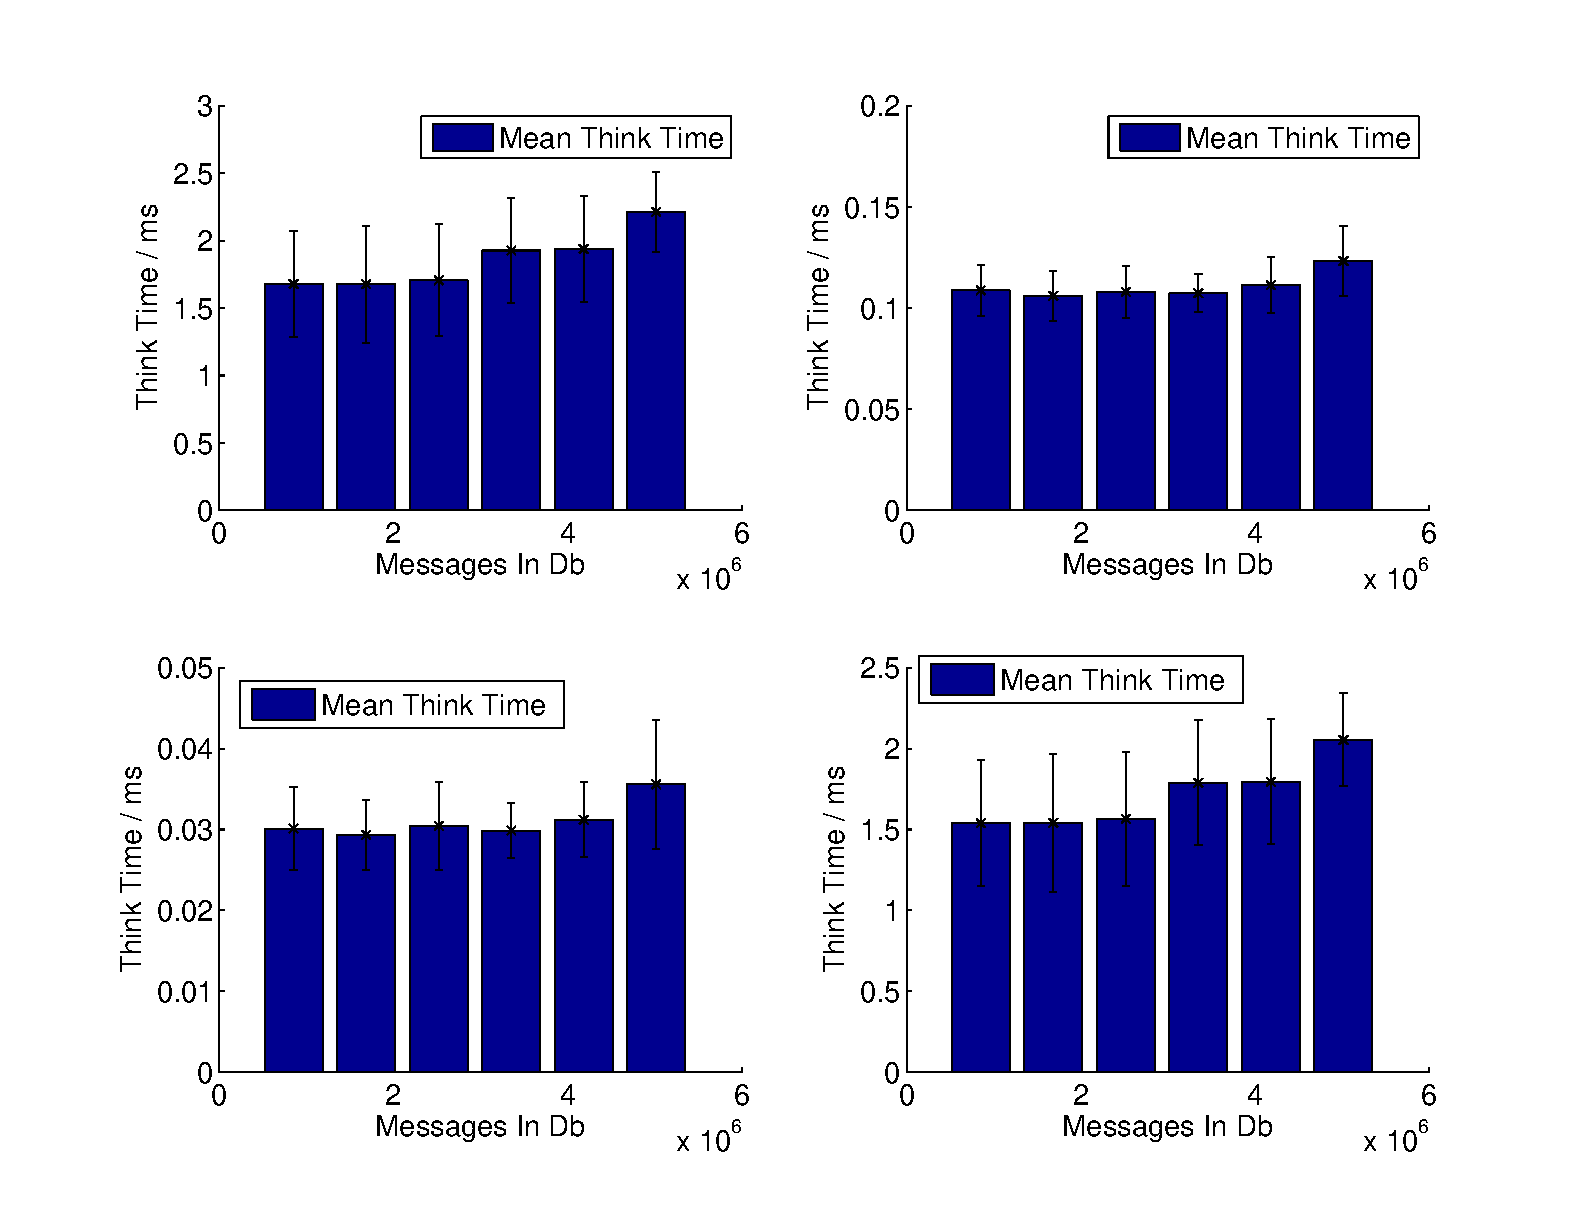
\includegraphics[scale=0.55]{resptime_as_function_of_msgs_in_db_push}}
                \caption{The response time as a function of number of messages in the database when performing sequential \textit{Send message}-requests using one (1) client and initially 20k messages in the database. The figure shows the total throughput (top left), think time in Socket I/O and job creation (top right), Client Request Worker (bottom left) and Persistence (bottom right)}
                \label{fig:resptime_as_function_of_msgs_in_db_push}
            \end{figure}
        The logs for this test can be found in \textit{micro-benchmarks/sequential\_requests}.

        \subsection{Difference in number of clients}
            The data needed for this test was gathered during the test described in Section \ref{sec:difference_in_size_of_dataset}. On Figure \ref{fig:msg_db_clients}, looking at tests with the same initial size of the dataset, we see that an increase in clients gives an increase in throughput in all of the tests.\\
            \\
            The logs for this test can be found in \textit{dataset-clients}.

        \subsection{Difference in frequency of requests}
            \label{sec:difference_in_frequency_of_requests}
            In this test we want to measure the impact on the server when we differ the frequency of requests. We performed 6 \textit{Send and Pop Same Client}-tests, differing only the wait time between requests. The tests were performed using one middleware with 30 database connections and 30 worker threads, and 100 client threads on the client machine.\\
            \\
            In this test we expect to see that the throughput increases with the number of requests, possibly reaching a point where it starts becoming unstable.\\
            \\
            On the left of Figure \ref{fig:sleep_time_between_requests_100clients_30_30} we see that the throughput increases as the wait time decreases, which is another way of saying that the throughput increases when the frequency of requests increases. We also see that the standard deviation increases slightly as the throughput decreases\\
            \\
            In the top right corner of the graph we see that the average time requests spend queuing in the middleware (waiting to get handed to a worker thread) is higher when the wait time between requests is zero.\\
            \\
            In the lower right corner we see that the combined time spent in Client Request Worker and IPersistence is going up when the frequency of requests increases.

             \begin{figure}[H]
                    \centering
                    \centerline{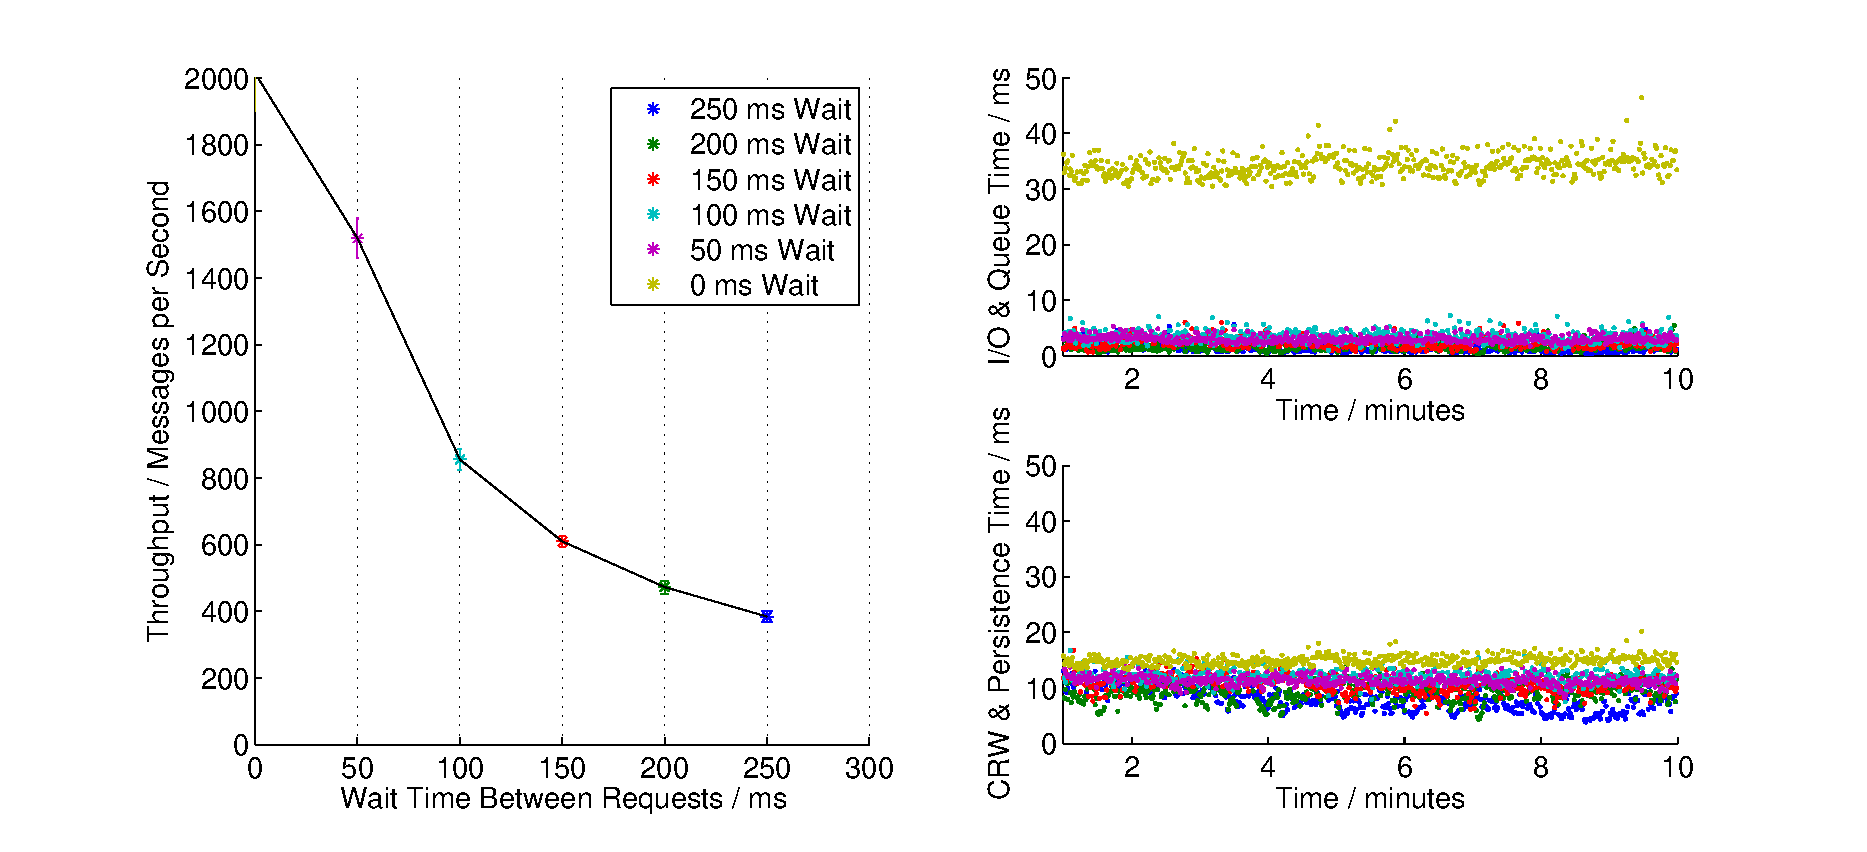
\includegraphics[scale=0.65]{sleep_time_between_requests_100clients_30_30}}
                    \caption{\textit{Send and Pop Same Client} test differing the amount of wait time between requests. On the left side we have plotted the throughput when increasing the wait time. In the top right corner we have plotted the average time of Socket IO \& Queue. In the lower right corner we have plotted the sum of \textit{IPersistence} and \textit{Client request worker}}
                    \label{fig:sleep_time_between_requests_100clients_30_30}
             \end{figure}
             ~\\
             \\
             On figure \ref{fig:sleep_time_between_requests_respTime_100clients_30_30} we see that the average response time goes up when we increase the frequency of requests. We also see that the standard deviation of response time decreases when the frequency of requests increases.\\
             \\
              \begin{figure}[H]
                      \centering
                      \centerline{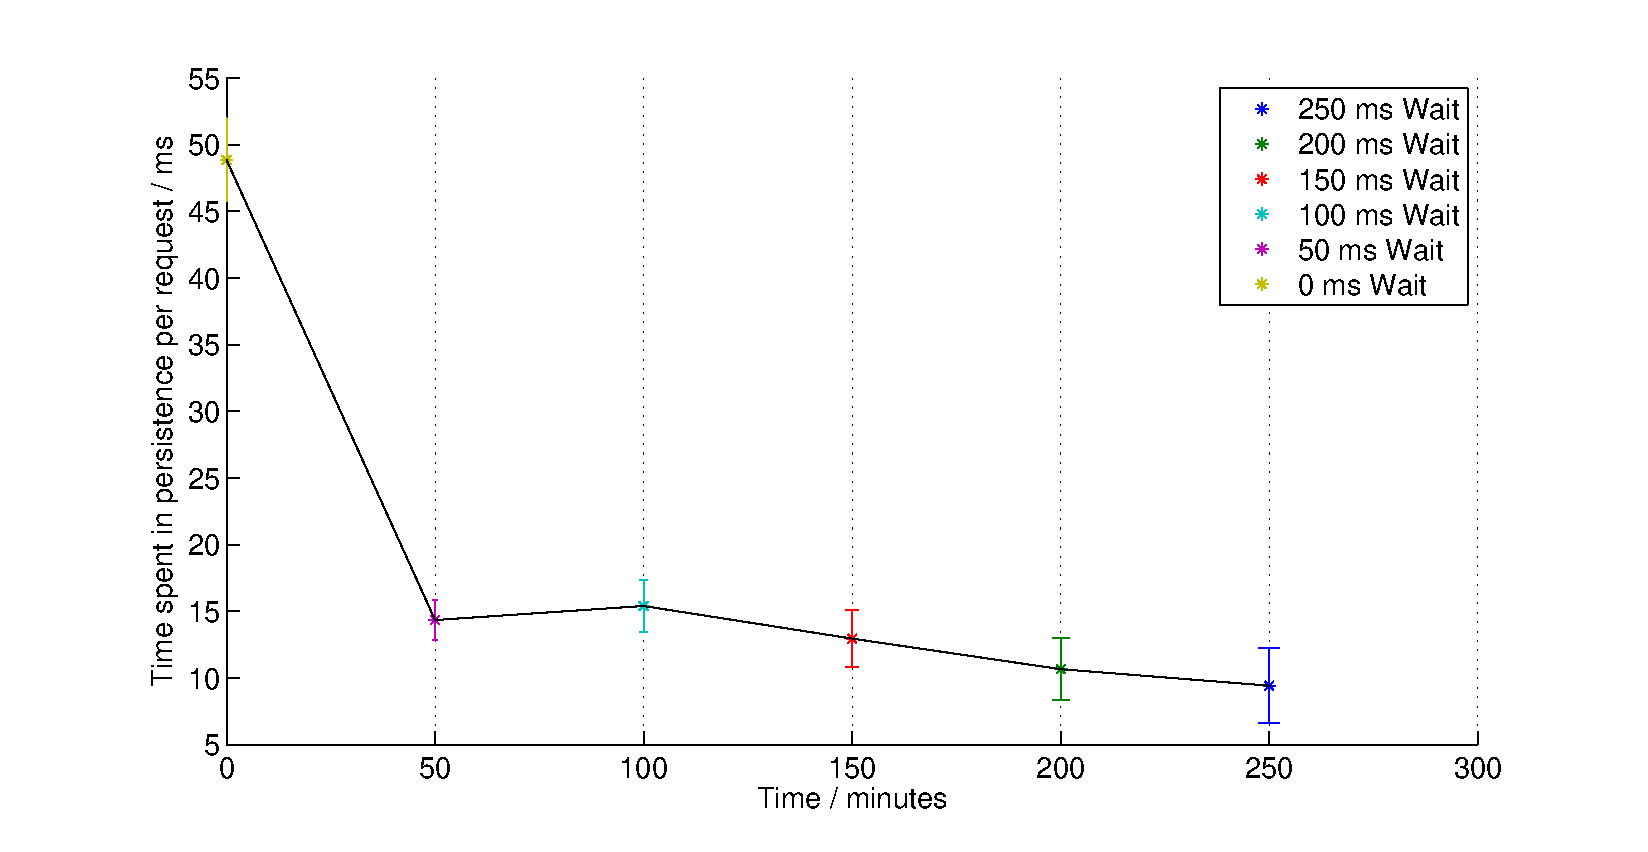
\includegraphics[scale=0.60]{sleep_time_between_requests_respTime_100clients_30_30}}
                      \caption{Same test as Figure \ref{fig:sleep_time_between_requests_100clients_30_30}, this time plotting total response time when increasing wait time}
                      \label{fig:sleep_time_between_requests_respTime_100clients_30_30}
              \end{figure}

        The logs for this test can be found in \textit{request-frequency}.

        \subsection{Difference in data store}
            In this test we measure the difference between using Postgres and not storing anything at all. We expect to see an an increase in throughput since we don't have to communicate with the database at all and thus don't have to wait for the network or database think time.
            
            \begin{figure}[H]
                \hspace{-1.5cm}
                \centerline{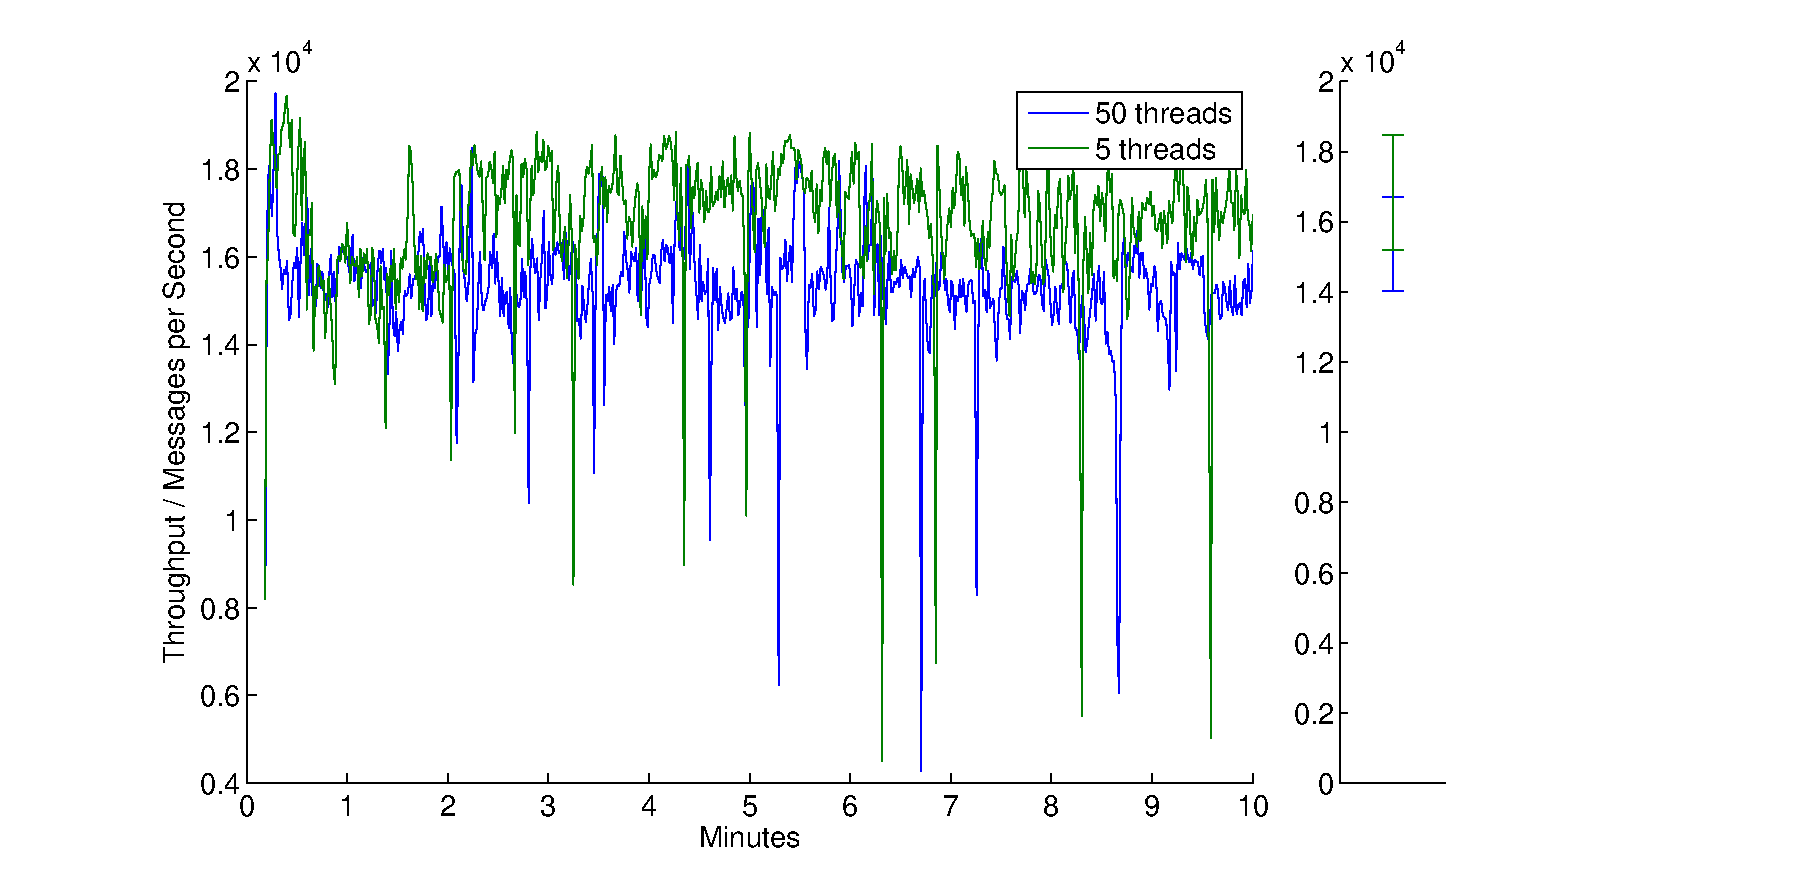
\includegraphics[scale=0.40]{throughput_i-fooled-you_50-5-threads-50-clients-1kB-msg}}
                \caption{The throughput when running \textit{SendAndPopSameClient} without any persistence and varying number of worker threads. Using 50 clients.}
                \label{fig:throughput_i-fooled-you_50-5-threads-50-clients-1kB-msg.eps}
                \end{figure}
            
            \begin{table}
            \begin{tabular}{|c|c|c|c|}
            \hline 
            Configuration & Mean Push Throughput & Mean Pop Throughput & Mean Response Time \\ 
            \hline 
            50 Threads & $8414.7 \pm 66.6$ & $8414.7 \pm 66.6$ & $1.30 \pm 0.01$ \\ 
            \hline 
            5 Threads & $8538.7 \pm 72.6$ & $8538.7 \pm 72.6$ & $1.24 \pm 0.01$ \\ 
            \hline 
            \end{tabular} 
                \caption{The throughput and response time data and confidence interval when running \textit{SendAndPopSameClient} without any persistence and varying number of worker threads. Using 50 clients.}
                \label{tbl:throughput_i-fooled-you_50-5-threads-50-clients-1kB-msg.eps}
            \end{table}

        The logs for this test can be found in \textit{no-persistence}.
            
        \subsection{Difference in number of middlewares}
        \label{sec:diff_middleware}
            \begin{figure}[H]
                \centerline{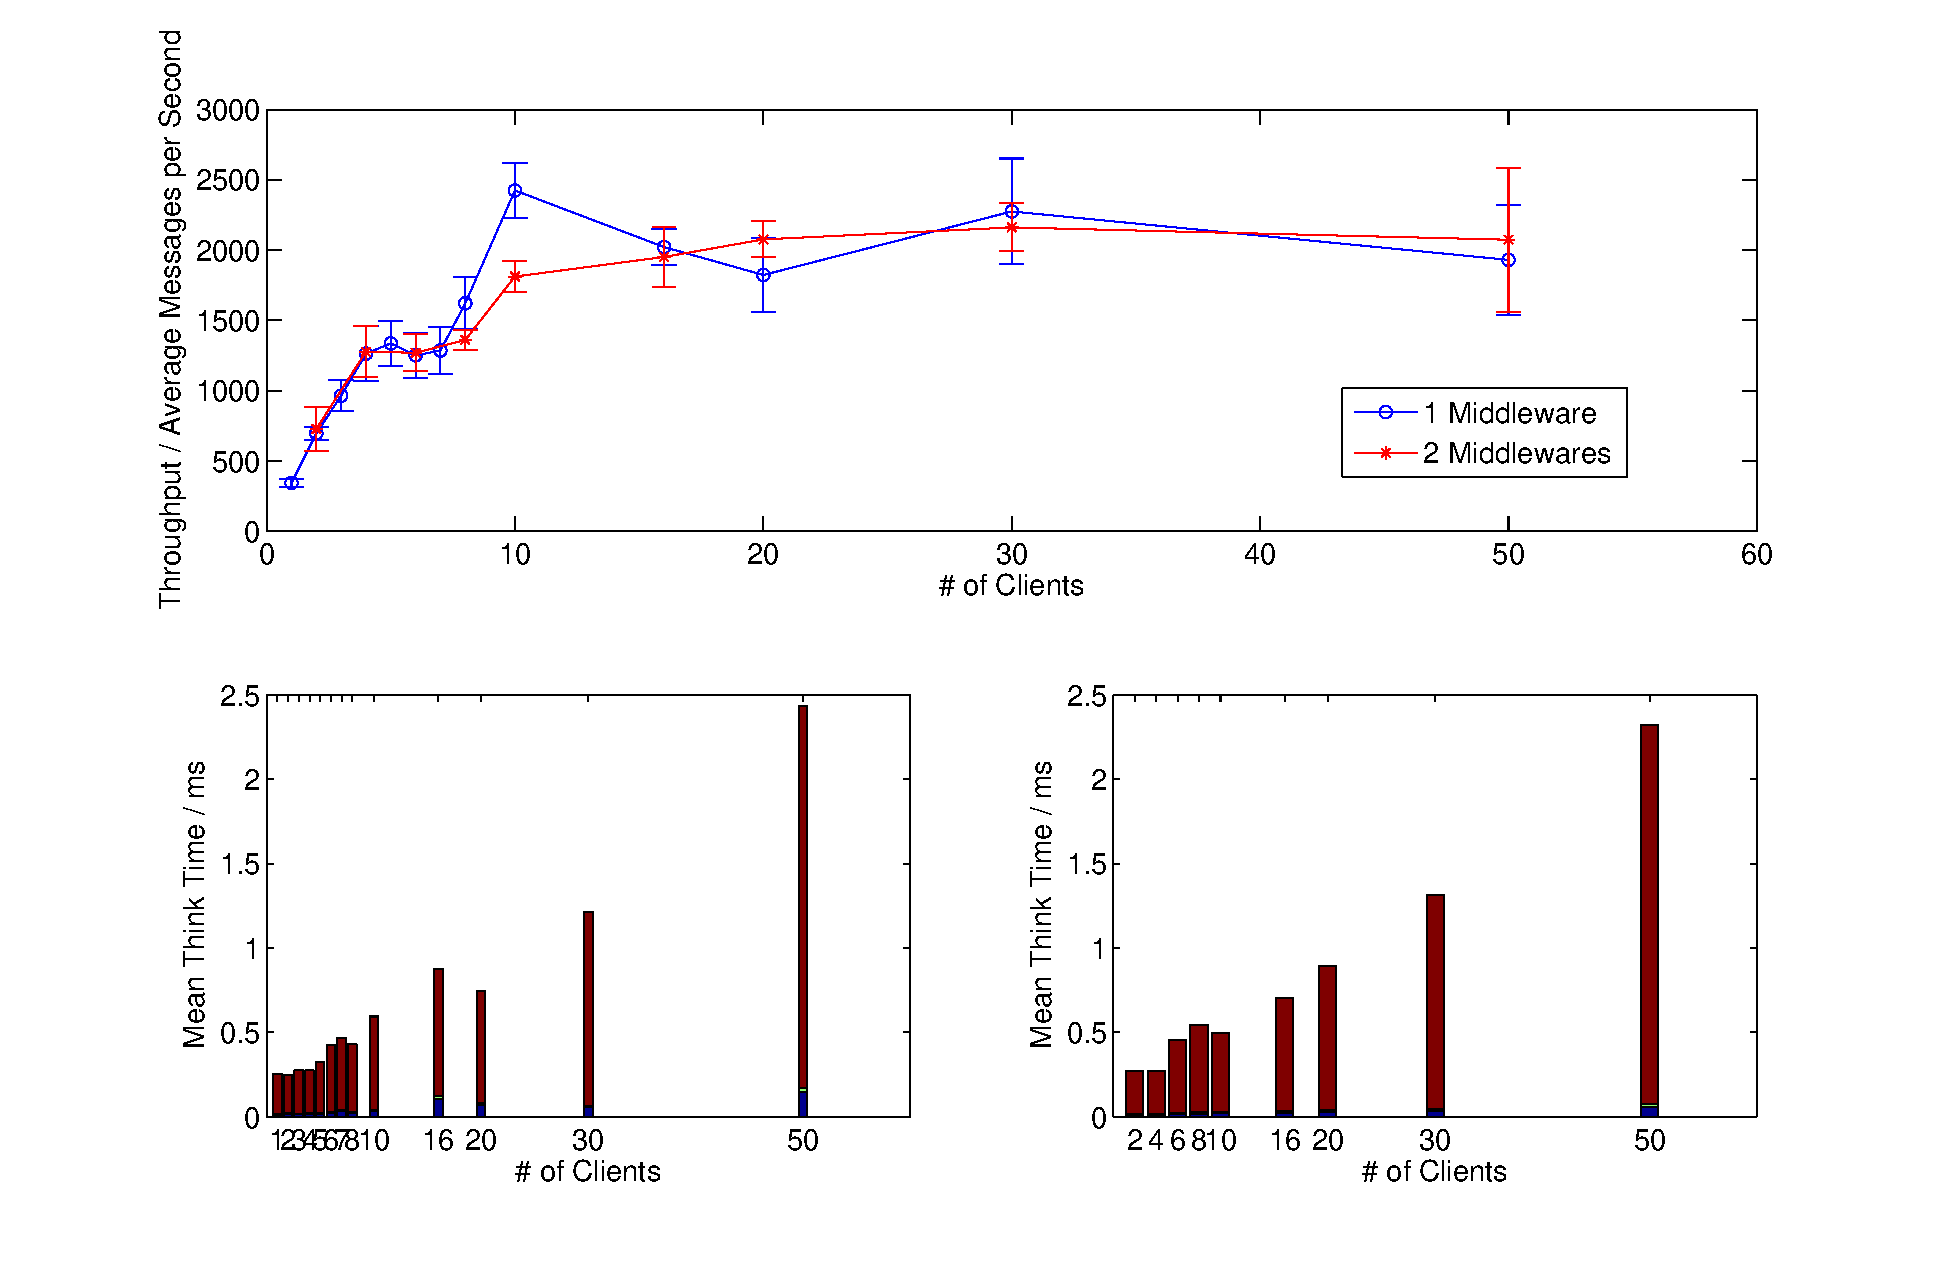
\includegraphics[scale=0.60]{throughout_middleware_clients}}
                \caption{The throughput when running \textit{SendAndPopSameClient} varying number of clients and number of middlewares.}
                \label{fig:throughput_middleware_clients}
            \end{figure}
            
            \begin{figure}[H]
                \centerline{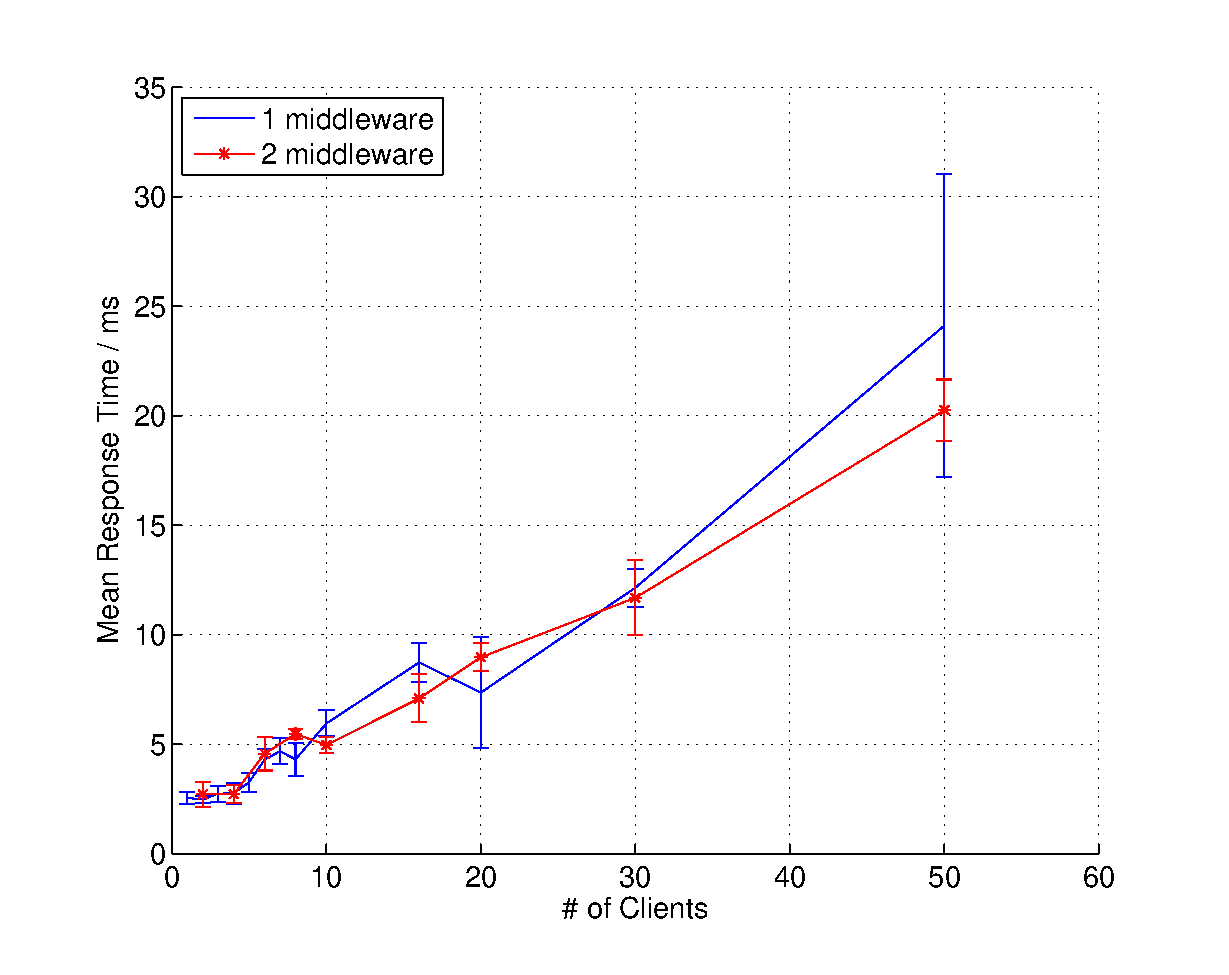
\includegraphics[scale=0.60]{throughout_middleware_clients_respTime}}
                \caption{The response time when running \textit{SendAndPopSameClient} varying number of clients and number of middlewares. The figure show response time increasing asymptotically after certain threshold.}
                \label{fig:throughout_middleware_clients_respTime}
            \end{figure}
            
            \begin{figure}[H]
                \centerline{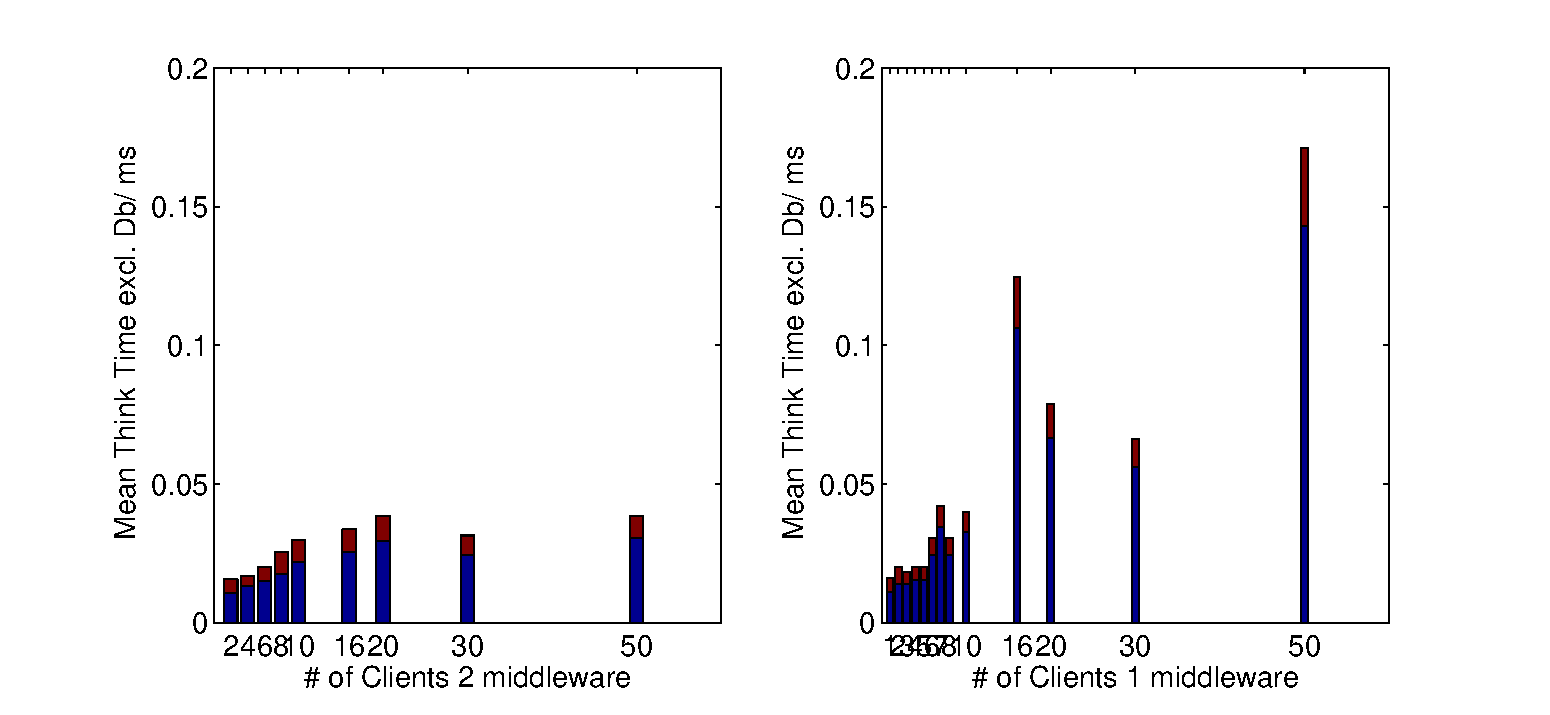
\includegraphics[scale=0.40]{throughout_middleware_clients_thinkTime_wo_db}}
                \caption{The mean think time excluding the persisting component for a request when varying number of clients and middleware.}
                \label{fig:throughout_middleware_clients_thinkTime_wo_db}
            \end{figure}

        The logs for this test can be found in \textit{middleware-scaleout}

        \subsection{1 vs 10 middlewares}    
            In this test with \textit{StandardTest} 1000 one-way clients and 500 two-way clients were used and the difference in performance when going form 1 middleware to 10 middlewares were measured.
            
            \begin{table}
            	\begin{tabular}{|c|c|c|c|}
            	\hline 
            	Configuration & Mean Push Throughput & Mean Pop Throughput & Mean Response Time \\ 
            	\hline 
            	10 Middlewares & $440.75  \pm 0.099$ & $2035.53 \pm 1.37$ & $11.55 \pm 0.11$ \\ 
            	\hline 
            	1 Middleware & $324.84 \pm 3.20$ & $2081.93 \pm 16.05$ & $44.55 \pm 0.49$ \\ 
            	\hline 
            	\end{tabular} 
                \caption{The difference in performance when using 1 and 10 middleware. It is clear that when increasing the middleware the response time decreases, while the total throughput  only increases marginally.}
                \label{tbl:differnce_1_and_10_mw}
            \end{table}
            
        The logs for this test can be found in \textit{1-vs-10-middleware}.


    	\subsection{Worker-threads vs Clients}
            In this test the Standard Test was run for 10 minutes with the purpose of finding the limit on where contention in the middleware would appear. The configuration that was used in this test was 1 middleware, varying the number of clients and the number of worker threads and database connections. This can be seen as a $2^k$ test even though number of clients, number of database connections and number of worker threads are both varied due to the result which was that the ratio should be 1:1 between the number of worker threads and number of database connections in the system for best performance. The results are presented in Table \ref{table:2k2-threads-clients}.
    		\begin{table}[H]
            \centerline{
    			\begin{tabular}{|c|c|c|c|}
    			\hline 
    			Configuration & Mean Push Throughput & Mean Pop Throughput & Mean Response Time \\ 
    			\hline 
    			100/100 + 500/250 & $335.95 \pm [-62.20, 70.30]$ & $2173.2  \pm  [-242.2, 265.0]$ & $113.16 \pm [-32.18, 36.47]$ \\ 
    			\hline 
    			100/100 + 300/125 & $147.39 \pm [-26.39, 28.95]$ & $1613.72 \pm [-115.92, 69.28]$ & $15.79 \pm [-6.6, 12.21]$ \\ 
    			\hline 
    			100/100 + 100/50 & $163.22 \pm [-9.22, 8.78]$ & $690.85 \pm [-16.85, 12.85]$ & $3.90 \pm [-0.87 , 1.71]$ \\ 
    			\hline 
    			30/30 + 500/250 & $325.95 \pm [-45.95, 51.05]$ & $1945.82 \pm [-165.72, 161.18 ]$ & $147.39 \pm [-26.39, 28.95]$ \\ 
    			\hline 
    			30/30 + 300/125 & $376.53 \pm [-43.63, 29.47]$ & $376.53 \pm [-43.63, 29.47]$ & $13.14 \pm [-7.14, 13.73]$ \\ 
    			\hline 
    			30/30 + 100/50 & $160.36 \pm [-12.36 , 2.83]$ & $638.58 \pm [-26.58, 19.12]$ & $5.40 \pm [-2.63, 2.83]$ \\ 
    			\hline 
    			\end{tabular}}
                \caption{Testing for number of clients and number of database connections and worker threads. The configuration that was used in this test was 1 middleware and the test was Standard Test. The notation in the configuration-columns is so that 1/2 + 3/4 means 1 database connection, 2 worker threads, 3 one-way clients and 4 two-way clients.} 
                \label{table:2k2-threads-clients}
            \end{table}
        The logs for this test can be found in \textit{threads-vs-clients}.

        \subsection{Difference in database connections and worker threads}
            \label{sec:difference_in_dbcons_and_worker_threads}
            In this test we perform 4 \textit{Send and Pop Same Client}-tests, differing the amount of worker threads and database connections. As explained in Section \ref{sec:description_middleware} we expect to see that the throughput of the middleware is bounded by the minimum of the number of worker threads and the number database connections.

             \begin{figure}[H]
                 \centering
                 \centerline{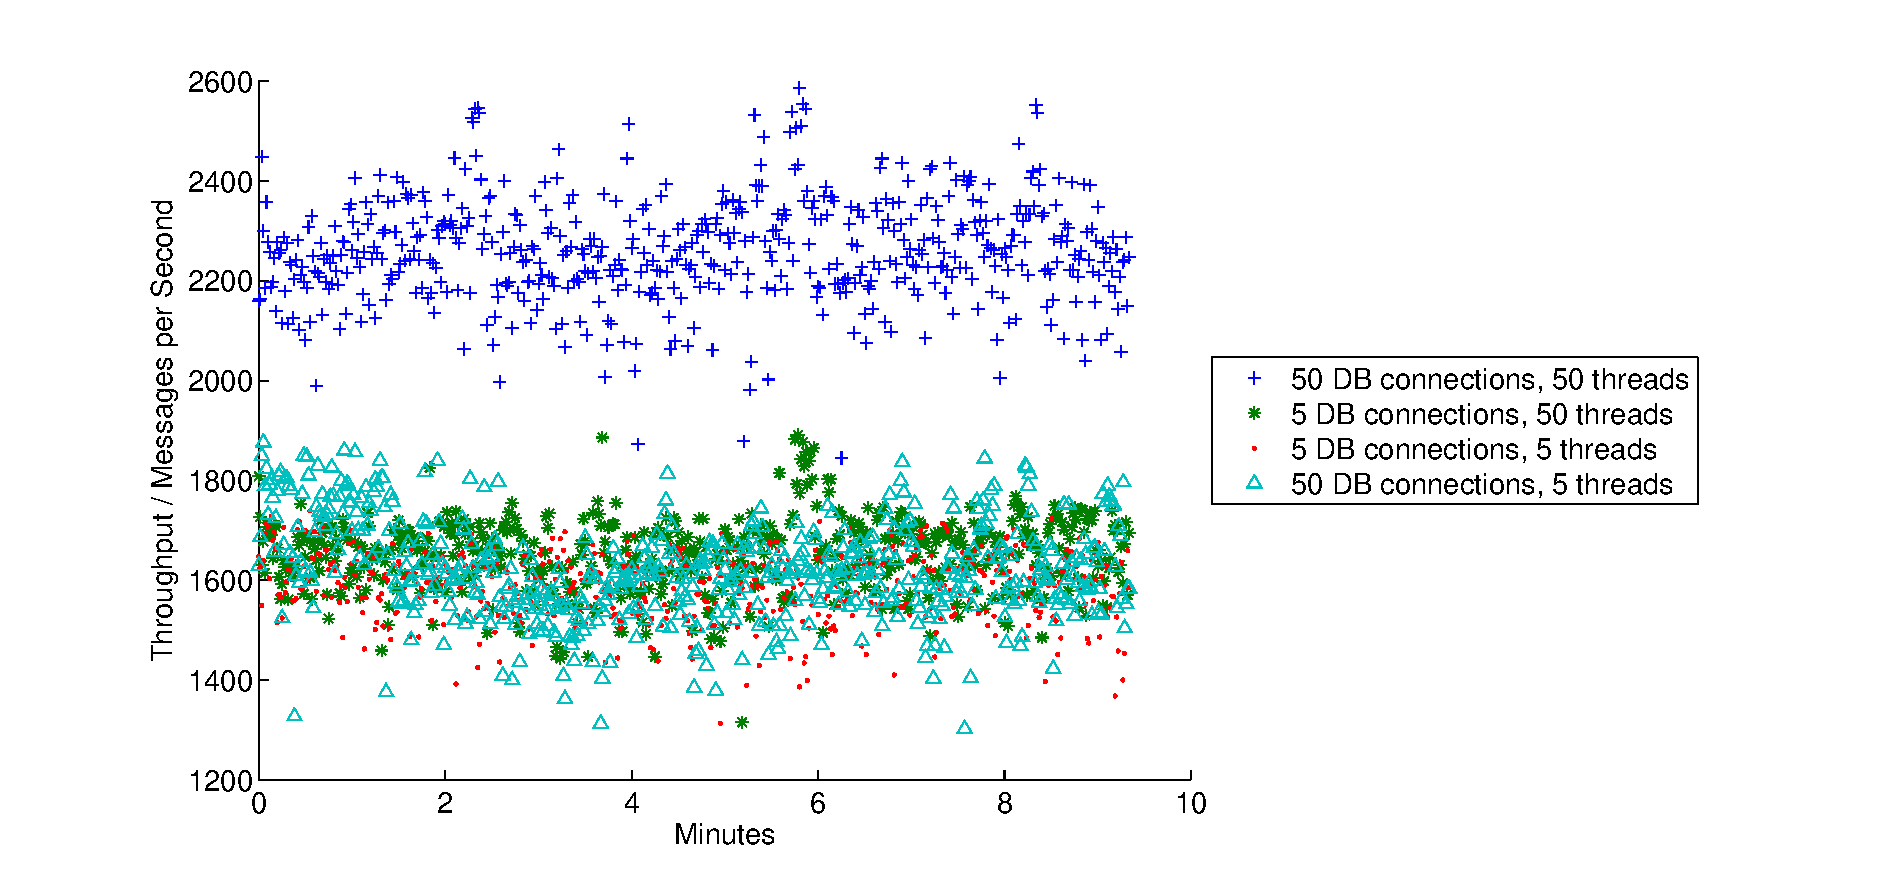
\includegraphics[scale=0.50]{throughput_vs_dbconns}}
                 \caption{The combined throughput of \textit{Send Message}- and \textit{Pop message} requests of the system while performing \textit{Send and Pop Same Client}, differing the number of database connections and worker threads on the middleware, performed on a single middleware.}
                 \label{fig:throughput_vs_dbconns}
             \end{figure}
             ~\\
             On Figure \ref{fig:throughput_vs_dbconns} we see that the result seems to be matching our expectations; the throughput is higher when both the number of database connections and worker threads is 50, but stays lower when either the number of database connections or worker threads is 5. Also we notice that the standard deviation of our results seem to increase as the maximum of the number of database connections and worker threads increases.
            % TODO: plot graphs for diff_worker-threads_client-threads-10db-cons-10ms-sleep and diff_worker-threads_client-threads-same-as-db-cons-10ms-sleep
            The raw data from these tests can be found in the log-folder, in the subfolders
            \begin{itemize}
                \item \textit{sendandpopsameclient\_diff\_worker-threads\_db-connections}
            \end{itemize}
            
        \subsection{Network Latency}
        \label{sec:network_latency}
        By performing 500 000 requests to the middleware and measuring the response time on the middleware and also on the client, we can calculate the network latency caused by the network by subtracting the mean response time of the client with the mean reasponse time on the middleware. The distribution of the response times can be seen in Figure \ref{fig:responsetime_dist_mw_and_client} and the measures difference can be seen in Table \ref{table:network_latency}.

            \begin{table}
                \begin{tabular}{|c|c|c|}
                    \hline 
                        MRT\footnote{Mean Response Time} on Client (ms) & MRT on Middleware (ms) & Mean Network Latency (ms)\\
                    \hline 
                        $4.358 \pm [-0.724, 0.915]$ & $3.957 \pm [-0.652, 0.696]$ & $0.402$ \\ 
                    \hline 
                \end{tabular} 
                \caption{Network Latency approximated by subtracting the mean response time on the server with the mean response time on the client.}
                \label{table:network_latency}
        \end{table}

        
        \begin{figure}[H]
                \centerline{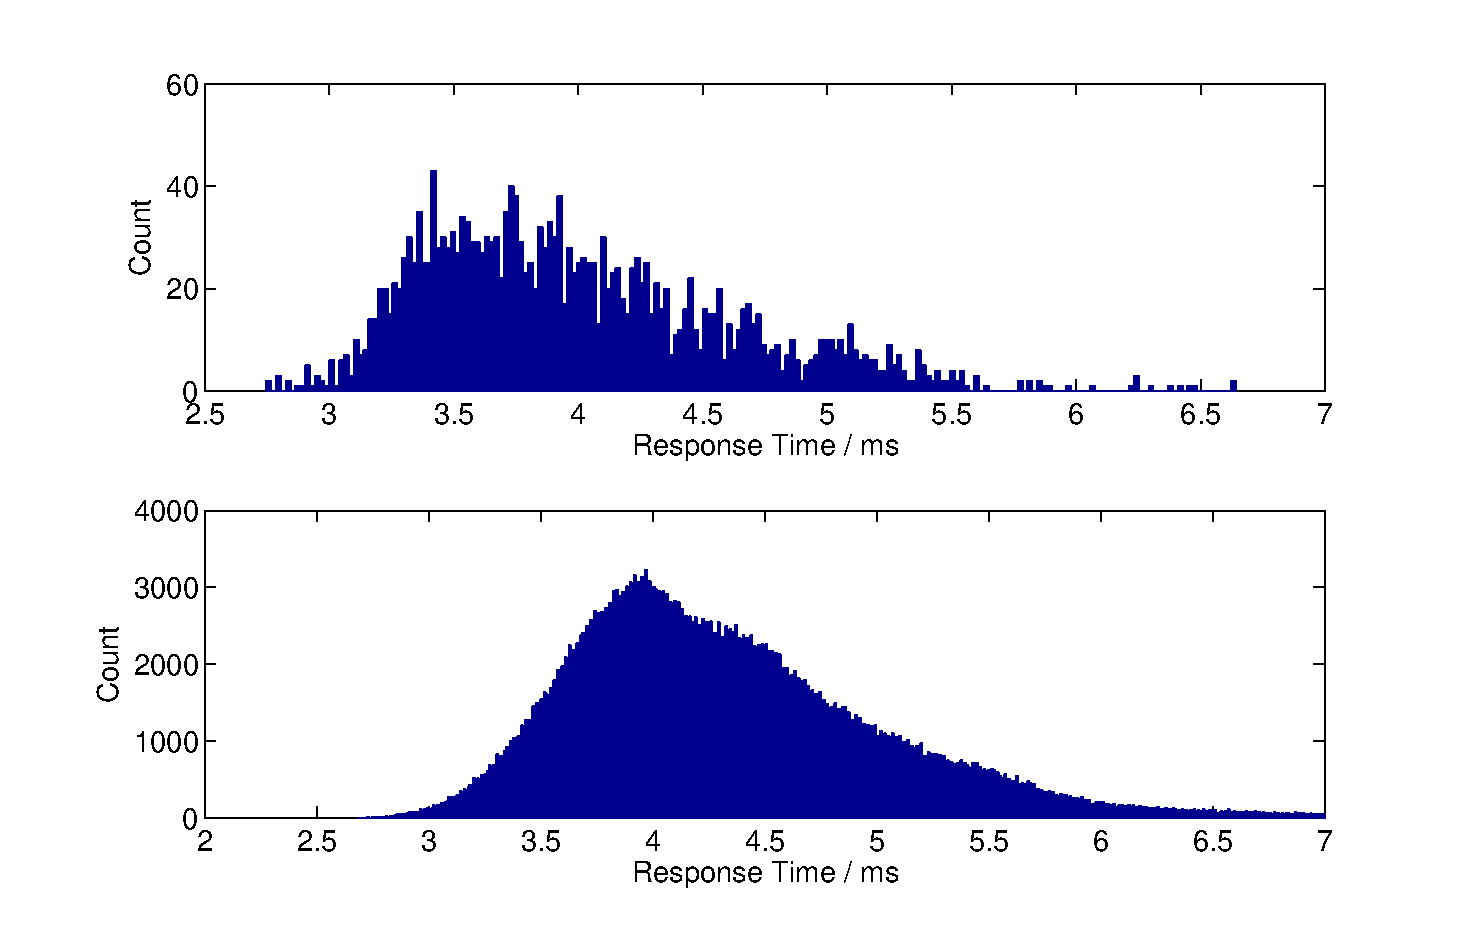
\includegraphics[scale=0.50]{responsetime_dist_mw_and_client}}
                \caption{The distribution of the response times on the middleware (top) and client (bottom). Sampled using 500 000 peek (as to not to vary number of messages in the system) requests to the middleware using one (1) client and more than 500,000 messages in the database.}
                \label{fig:responsetime_dist_mw_and_client}
        \end{figure}
            
 
        The logs for this test can be found in \textit{micro-benchmarks/sequential\_requests}.
        \subsection{Neighbour Noise} 
        As discussed in Section \ref{sec:tests_and_results}, all our deployments live on a cloud hosting platform and thus are subject to neighbour noise. To demonstrate that the difference in computing power avaiable to our system varies over time an identical test were run on the evening (around 20:00) on day, and once again in the morning the next day (around 10:00). The difference in throughput and response time is presented in Figure \ref{fig:same_test_different_time_of_day} and \ref{fig:same_test_different_time_of_day_resp_time_over_time}.

    
        \begin{figure}[H]
                \centerline{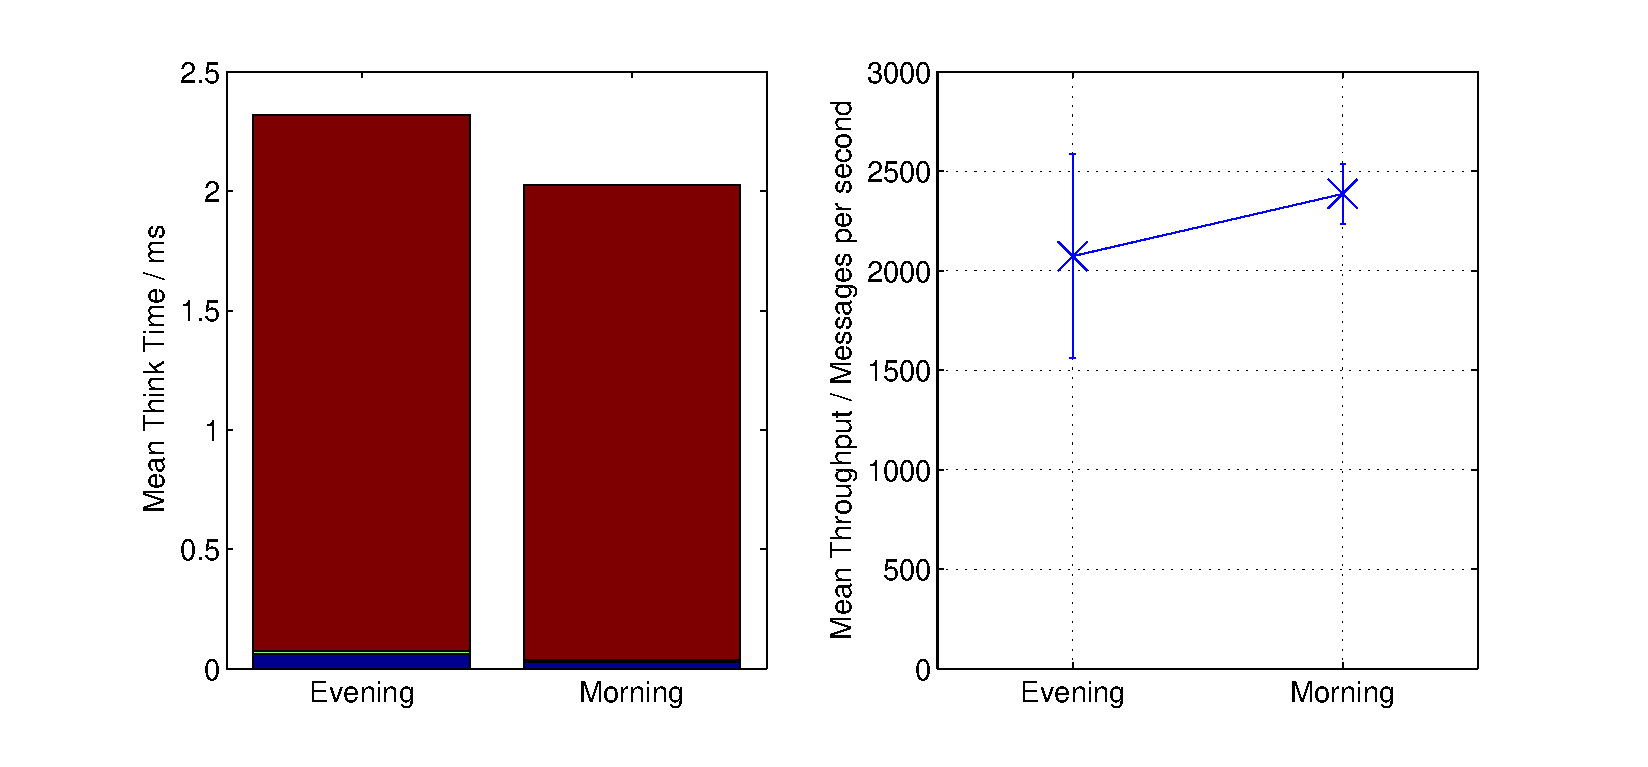
\includegraphics[scale=0.50]{same_test_different_time_of_day}}
                \caption{The mean think time and mean throughput for the same test run at two different times under the day using exactly the same configuration. Run 1 was run at the evening around 20:00 and Run 2 was run in the morning around 10:00.}
                \label{fig:same_test_different_time_of_day}
        \end{figure}
    
        \begin{figure}[H]
                \centerline{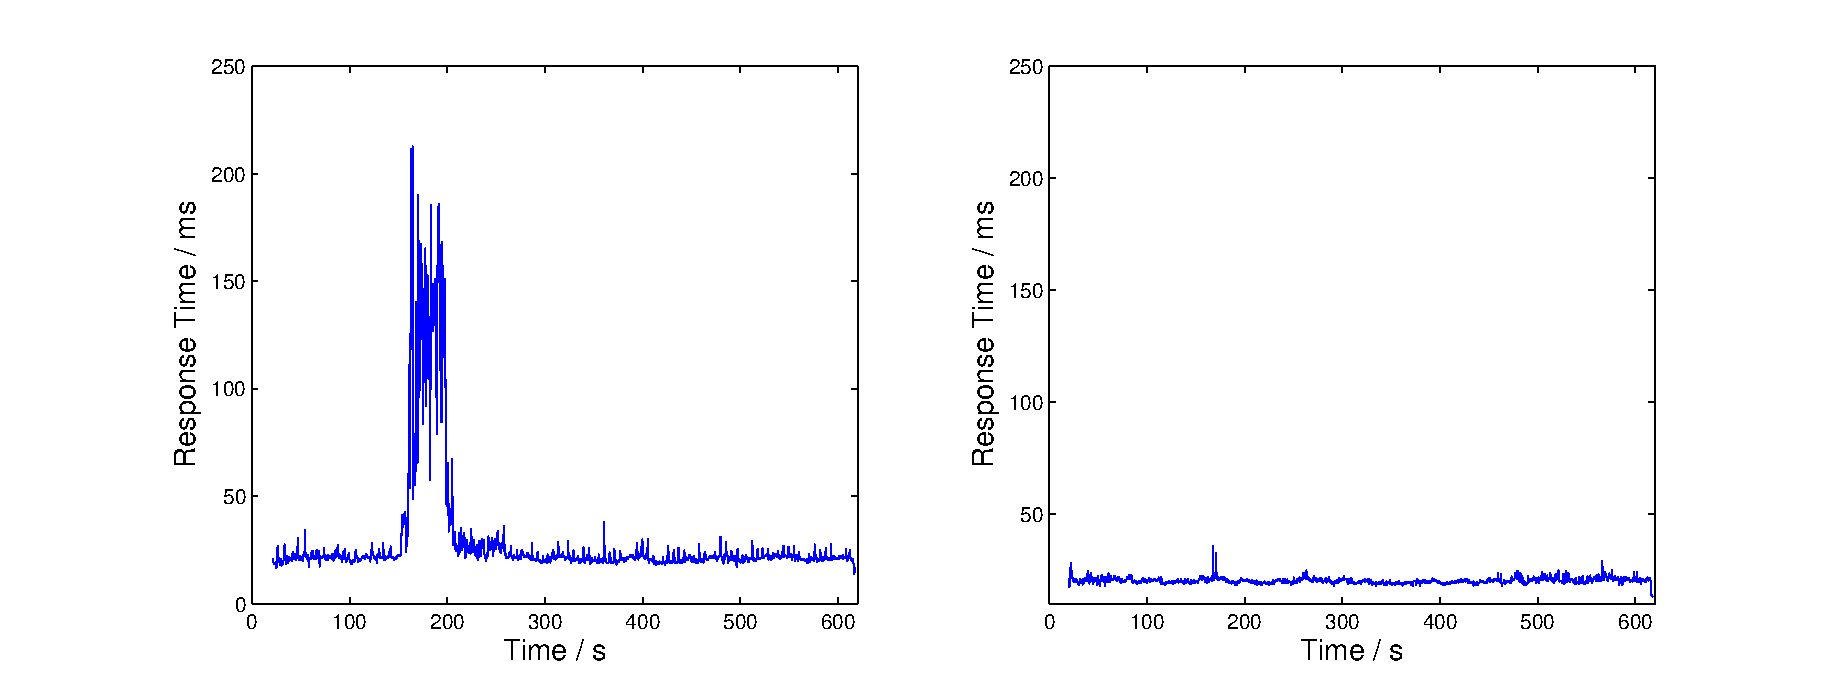
\includegraphics[scale=0.50]{same_test_different_time_of_day_resp_time_over_time}}
                \caption{The response time over time for the same test run at two different times under the day using exactly the same configuration. The left figure shows the test that was run at the evening around 20:00 and the right was run in the morning around 10:00.}
                \label{fig:same_test_different_time_of_day_resp_time_over_time}
        \end{figure}

    The logs for this test cane be found in \textit{same-test-differente-times}
    \section{Analysis}
        \label{sec:analysis}
        In this section we interpret and compare the results shown in Section \ref{sec:tests_and_results} above, in order to figure out what the different performance metrics of our system are.

        \subsection{Time spent in each part of the system}
            \label{sec:time_spent_in_each_part_of_the_system}
            % TODO USE DATA FROM diff_db-cons_worker-threads_i-fooled-you VS diff_num-db-threads AS WELL
            In order to determine how much time is spent in each part of our system, we look at the results we measured during code profiling (Figure \ref{fig:code_profiling_send_pop_same_client} and \ref{fig:code_profiling_standard_test}) and the data we have on the bottom of Figure \ref{fig:throughput_middleware_clients}.\\
            \\
            The results of our code profiling show that 83-87\% of our codes' execution time is spent waiting for replies from the database. It is important to note that this time \textit{includes the network delay} between the middleware and the database, in both directions.\\
            The results from the code profiling are backed up with our own logging data, where we have also measured how much time is spent in different parts of our system. On Figure \ref{fig:throughput_middleware_clients} we also have evidence that the server spends most of its time waiting for a response from the database, waiting in the IPersistence class of our implementation. Assuming that the VisualVM tool is correct this confirms that our measuring techniques employed are valid.\\
            \\
            This data all points to the database or the network being the bottleneck in these particular tests. We contribute this to choosing bad indexes for our data, having a poorly configured database, or having a slow network. The slow network is though very unlikely, since from what we can deduce from Section \ref{sec:network_latency} the network latency is very small (around 0.5ms) and we observe think times in the persistence component bounded by around 1.5 from below, see Figure \ref{fig:thinktime_push_peek_pop}. We also get a much higher throughput when not storing any messages at all (i.e. the \textit{I Fooled You} persistence implementation), as seen in Figure \ref{fig:throughout_middleware_clients_thinkTime_wo_db}, where we have a throughput of around 17k messages per second and a response time of around 1.3 ms.

            % DONE!!!!! ?



            % USE:
            %   1) diff_db-cons_worker-threads_i-fooled-you VS diff_num-db-threads
            %   2) Use Network Latency Client<->MW
            %   2) Code profiling above
            %   3) Plots showing CRW, IO, and DB
            % SHOW:
            %   1 -> we have WAY better performance with i_fooled_you
            %   2 -> our profiling shows that we spend WAY more time doing db-stuff than anything else
            %   3 -> our measurements show that we wait a lot for the database, compared to anything else
            % CONCLUDE:
            %   We spend a lot of time in the database, which might be because of bad configuration, indexes etc.


        \subsection{Size of messages}
            We can see from Figure \ref{fig:responsetime_msgsize} that the size of a message only affects the time to perform \textit{Send message}. \textit{Pop message} and \textit{Peek message} seem unaffected by the size of the message. This is attributed to the fact that the database has to push data to disk (whether it's the write-ahead-log or the actual data) in order to promise durability, whereas it's possible not to hit disk when reading data from memory. We draw the conclusion that our system handles big payloads well.


            % USE: 
            %   1) diff_clients_msgsize-10b VS diff_clients_msgsize-1mb VS diff_clients_msgsize-10mb
            %   2) fig:responsetime_msgsize
            % SHOW:
            %   1 -> it doesn't seem to matter much
            %   2 -> it seems to matter for push
            % CONCLUDE:
            %   THIS MIGHT BE A BIT TOO CONTRIVED:
            %   We have one component that performs so poorly that our other configurations don't really seem to matter

        \subsection{Number of middlewares}
            % USE
            %   1) fig:throughput_middleware_clients
            %   2) response time data from test in 1)
            % SHOW:
            %   1 & 2 -> throughput increases with the number of clients
            %   1 & 2 -> response time decreases with the number of middleware. This is because of #worker-threads which limits the amount of simultaneous requests.
		   In Figure \ref{fig:throughput_middleware_clients} it is shown that when we increase the number of clients across one and two middleware, they hit the throughput threshold at the number of clients. We can also see in Figure \ref{fig:throughout_middleware_clients_thinkTime_wo_db} that while the throughput is the same for the system and the response time is increasing with the same amount (Figure \ref{fig:throughout_middleware_clients_respTime}) the response time excluding the persistence component is increasing more for each additional client when running 1 middleware relative to distributing the clients to 2 middlewares. This shows that while the system on the middleware is less stressed, the think time in the database, which is the bottleneck in the whole system, is increasing for both configurations (1 vs 2 middleware). One can also see a tendency to the system with two middlewares having a slightly shorter response time overall -- which is expected (Figure \ref{fig:throughout_middleware_clients_respTime}). We can also see that the throughput will flatten out after a certain threshold, and that this threshold is the same as for when the response time start to behave asymptotically.

        \subsection{Number of clients}
        When increasing the number of clients (which perform the \textit{Standard Test}, i.e. is interacting with the system) to a middleware we see that the throughput increases, see Figure \ref{table:2k2-threads-clients}. This is expected behavior, as is the observation that the system has an upper limit on the throughput and thus the number of clients connected the middleware. When this limit is hit, adding more clients to the middleware will not lead to an increased throughput, just increase response time.


        \subsection{Stability of the system}
            In our long trace test we saw that our system behaved in a reasonably stable manner over the four hour test.\\
            \\
            When comparing the throughput and the response times in Table \ref{table:2k2-threads-clients} for 750 clients, 100 worker threads and 750 clients, 30 worker threads, we see that the throughput stays about the same and that the response time goes up. From this we can see that the increase in clients means that queues are building up in the middleware. Even when we have queues in the middleware, we see that the system behaves in a stable manner.\\
            \\
            When we compare the throughput from when 150 client and 100 worker threads were used, and 750 clients and 100 worker threads we see that the throughput is increasing when the number of clients increases. We see that the confidence interval (again, see numbers in Table \ref{table:2k2-threads-clients}) increases heavily. This increase in the confidence interval shows that we are pushing the system a lot more with 750 clients than we do with 150 clients. The narrow confidence interval we have with 150 clients shows that we aren't pushing the system to the point of making it unstable, but that we are on our way to this point when we use 750 clients. \\
            \\

        \subsection{Frequency of requests}
            \label{sec:frequency_of_requests}
            % USE
            %   'Difference in number of clients'
            %   'Differency in frequency of requests'
            % SHOW
            %   We've shown that the system didn't reach its' limit yet, but the big deviation we get with many requests (many clients) shows that we might reach that point
            As noted in Section \ref{sec:difference_in_frequency_of_requests} we see on Figure \ref{fig:sleep_time_between_requests_100clients_30_30} that the throughput of our system goes up when the frequency of requests increases. This seems reasonable, and points to the fact that our system can handle more load than the test produces when the wait time is relatively high. What seemed to be counter-intuitive to us in the beginning was that the average response time (as shown on Figure \ref{fig:sleep_time_between_requests_respTime_100clients_30_30}) is much higher when the wait time is lower, even though the throughput is much higher at the same time. After plotting the top right part of Figure \ref{fig:sleep_time_between_requests_100clients_30_30}, we realized that this must be because there are many requests queued, waiting to be served. This gives a higher throughput since the server always has a new request to process and at the same time gives a higher average response time since there are requests waiting to be served in the queue.\\
            \\
            As we also noted in Section \ref{sec:difference_in_frequency_of_requests} the standard deviation of response time becomes higher as the average response time becomes lower, and the frequency of messages decreases. What's believed to be happening at this point is that the requests are so infrequent that there is (almost) no queuing in the middleware, causing requests to be processed immediately. When the average response time becomes as low as 10 milliseconds, it is seems very reasonable to us that the standard deviation increases, since things such as network i/o will play a big part in the result.\\
            \\
            Finally we note that our system seems to be performing best (in this particular setup) when the wait time between requests is around 50-60 milliseconds, an average of 1500-1600 requests per second (when the distribution of requests is half \textit{Pop message} and half \textit{Send message}), since this is the point where the throughput is relatively high while the average response time hasn't begun increasing drastically yet.

        \subsection{Bounded throughput caused by middleware configuration}
            \label{sec:analysis_bound_on_throughput}
            On Figure \ref{fig:throughput_vs_dbconns} we saw that, as per our expectations, the throughput of the middleware (assuming a high enough frequency of requests) is bounded by the minimum of the number of database connections and the number of worker threads. This is a very intuitive result since each worker thread will use exactly one database connection per (well-formed\footnote{I.e. not an invalid request or a request that is not a handshake request.}) request. This means that if we want to keep the utilization of both worker threads and database connections high, we should keep the ratio between them 1, as other ratios would leave one of the resources idle.\\
            This result is backed up by the results of our long traces where, in Table \ref{table:2k2-threads-clients} and \ref{table:2k2-threads-clients}, we saw that increasing the amount of database connections and worker threads also resulted in a higher standard deviation in throughput.\\
            \\
            In both of the mentioned tests we also see that the standard deviation of the results seems to be increasing when the amount of worker threads and database connections is increased. We attribute this to the fact that we give the database more work to do simultaneously, causing a higher response time for the database.\\
            \\
            If we look at the measured think-time of the database during the long traces, we see that this confirms our suspicion; the think-time of the database increases when we increase the amount of worker threads and database threads.

        \subsection{Micro benchmarks}
            \label{sec:analysis_micro_benchmarks}
            The response time patterns for the pop request showed in Figure \ref{fig:responsetime_500k_pop} is a strange pattern that seems to be caused by the decreasing the number of messages in the database cause by the pop calls themselves. This is concluded since the pattern does now show up when only peeking and not thus now varying the number of messages in the database. It seems that some external factor might be causing this, for instance we have Postgres' automatic VACUUM activated. It could be that the trend we see decreases because the number of messages in the database decrease and that the VACUUM operation therefore takes less time.\\
            \\
            In section \ref{sec:micro_send_message} we see that the average response time of \textit{Pop message} is around twice that of \textit{Peek message}. This is explained by the fact that we, as described in \ref{sec:description_middleware}, in our implementation of \textit{Pop message} in the middleware, make a call to \textit{Peek message} and if a message is returned we make a call to delete the this message from the database. This means that we send two requests to the database for all \textit{Pop message} requests that finds a message requested by the client.\\
            \\
            We also see that the response time for popping is decreasing when the number of messages in the database is decreasing (see Figure \ref{fig:resptime_as_function_of_msgs_in_db_pop}), and we see the inverted pattern when pushing messages, i.e. the response time for pushing is increasing when the number of messages in the database is increasing (see Figure \ref{fig:resptime_as_function_of_msgs_in_db_push}). When peeking, the response time stays constant withing the standard deviation (see Figure \ref{fig:resptime_as_function_of_msgs_in_db_peek}).

    \section{Conclusion}
        % More middleware does not increase throughput because the database is the bottle neck, and is shared among all middleware.
        % Increasing # middleware can give a lower response time, if there are enough requests (vs worker threads and db cons) to form queues in the middleware

        In Section \ref{sec:difference_in_dbcons_and_worker_threads} we found that the performance of our middleware depends, among other things, on the ratio between the amount of worker threads and database connections. In this section we found that the ratio should be 1 if we want to utilize all of our database connections and worker threads simultaneously. This was a very intuitive result to us, and was exactly what we expected to see.\\
        \\
        Not only does the ratio between worker threads and database connections matter, so does the \textit{number} of worker threads and database connections. We can see this when having a saturated system with 30 worker threads and 30 db connections, and then increasing number of worker threads to 100 and db connections to 100 also. Here we can see (Table \ref{table:2k2-threads-clients}) that the throughput increase is not statistically significant (stays within standard deviation) but the response time is decreased.\\
        \\
        In our analysis in Section \ref{sec:time_spent_in_each_part_of_the_system} we found that found that during execution of our middleware, most of the time is spent waiting in the persistence component or, more specifically, waiting for responses from the database. This result is consistent with the test results from the other tests we made that put a significant load on the system. This implies that, in our current setup, the database is the bottleneck. We do not blame this on the database implementation, but rather on ourselves, for choosing bad indexes and/or configuring the database poorly w.r.t. the dataset we have and the type of queries our middleware performs.\\
        If we had had more time to test our system we would try to change the indexes and rerun our tests to see how much performance we could gain from a more appropriate configuration of the database. This is also further confirmed by the scaling up test (see Section \ref{sec:diff_middleware}) where increasing the number of middlewares did not increase the throughput. This is expected when the database is the bottleneck since this is a shared resource between the middlewares, and when this is the limiting device for throughput then it does not matter how many middlewares are used.\\
        \\
        The maximum throughput is around $2500 \pm 300$ requests per second for the \textit{Standard Test}, and around $2000 \pm 210$ requests per second for \textit{Send and Pop Same Client}.\\
        We found that we got the best performance with the \textit{Send and Pop Same client} test when there are around 1500 requests per second, since this is where the throughput is the highest while the response time is still as low as 15 milliseconds (See Figure \ref{fig:sleep_time_between_requests_100clients_30_30} and \ref{fig:sleep_time_between_requests_100clients_30_30}).
        % TODO: 
        % TODO: It's better to have more worker threads, but only up to a certain point. We have data that shows that it's better to have 30 worker threads than 100 in some situations
    \clearpage
    \appendix
        \section{Message protocol and API}
        \label{sec:message_protocol_api}
            \subsection{Exceptions}
                If a request cannot be fulfilled by the server, the server will respond with an exception.  Exceptions have the following format:\\
                \\
                \indent\textit{FAIL $<$type$>$ $<$id$>$}\\
                \\
                Where $<$type$>$ is either QUEUE, CLIENT, MESSAGE, or UNKNOWN, and where $<$id$>$ is the id of the queue, client or message that ‘failed’. For instance, if a client tries to send a message to the queue with id 5 and if that queue doesn’t exist, the server will respond with “FAIL QUEUE 5”.

            \subsection{Handshake}
                The client should send HELLO when first connecting to the server. The server should respond with OK if it accepts the client, otherwise the server should respond with something else. The client must disconnect if it receives anything other than OK from the server.


            \subsection{Send Message}
                \indent\indent\textit{MSG,ReceiverId,SenderId,QueueId,Priority,Context,Content}\\
                \\
                \textbf{Response}\\
                The server should respond with OK if the message was inserted into the queue successfully, otherwise it should respond with FAIL.\\
                \\
                \textbf{Remarks}\\
                To send a message to multiple queues, separate the QueueIds with a semicolon, e.g. 1;2;3 to send the message to queues 1, 2 and 3.

            \subsection{Message Response}
                \indent\indent\textit{MSG,SenderId,Context,MessageId,Content}\\
                \\
                This is here to save space in the definitions below. This is how the server should return a message upon request from the client.

            \subsection{Peek Queue}
                \indent\indent \textit{PEEKQ,ReceiverId,QueueId,OrderByTimestampInsteadPriority}\\
                \\
                \textbf{Response}\\
                The server should respond with the message formatted as in section A.4 if there is a message in the queue. Otherwise the response should be MSG0.\\
                \textbf{Remarks}\\
                OrderByTimestampInsteadPriority is either 1 or 0.

            \subsection{Peek Queue with Specific Sender}
                \indent\indent\textit{PEEKS,ReceiverId,QueueId,SenderId,OrderByTimestampInsteadPriority}\\
            \\
            \textbf{Response}\\
            The server should respond with the message formatted as in section A.4 if there is a message in the queue. Otherwise the response should be MSG0.\\
            \\
            \textbf{Remarks}\\
            OrderByTimestampInsteadPriority is either 1 or 0.


            \subsection{Pop Queue}
                \indent\indent\textit{POPQ,ReceiverId,QueueId,OrderByTimestampInsteadPriority}\\
                \\
                \textbf{Response}\\
                The server should respond with the message formatted as in section A.4 if there is a message in the queue. Otherwise the response should be MSG0.\\
                \\
                \textbf{Remarks}\\
                OrderByTimestampInsteadPriority is either 1 or 0.

            \subsection{Pop Queue with Specific Sender}
                \indent\indent\textit{POPS,ReceiverId,QueueId,SenderId,OrderByTimestampInsteadPriority}\\
                \\
                \textbf{Response}\\
                The server should respond with the message formatted as in section A.4 if there is a message in the queue. Otherwise the response should be MSG0.\\
                \\
                \textbf{Remarks}\\
                OrderByTimestampInsteadPriority is either 1 or 0.

            \subsection{Create Queue}
                \indent\indent\textit{CREATEQUEUE,NameOfQueue}\\
                \\
                \textbf{Response}\\
                The server should respond with the id (long) of the queue, if a queue with the same name exists the server should respond with FAIL.

            \subsection{Remove Queue}
                \indent\indent\textit{REMOVEQUEUE,QueueId}\\
                \\
                \textbf{Response}\\
                The server should respond with OK or FAIL.

        \section{Log Files}
        In our tests we logged both at the client and at the client side. This section goes through how to parse the log files.

            \subsection{Middleware Logs}
            The middleware log on a set interval which can be configured in a configuration file which is read once at startup by the middleware, and each time this interval is hit, this is added to the log:
            \begin{lstlisting}[breaklines]
            [milliseconds since middleware start], [count of push requests], [count of pop/peek requests], [total number of requests received], [total time in Socket IO], [total time in CRW], [total time in persistence]
            \end{lstlisting}
            Note: All logged data except the first column is reset for each logging event. So the count of push requests is the count of push requests since $t-\Delta t$ where $\Delta t$ is the logging interval. Also note that Socket IO includes the amout of time the request spends in waiting in for a free worker thread.


            \subsection{Client Logs}
            The log files used in the tests described in this test have the follow formatting, and is logged every time a request finishes:
            \begin{lstlisting}[breaklines]
            [milliseconds since client start], [duration of request]
            \end{lstlisting}

        \section{Sample Distributions}
        Here are some figures over the distributions of some of the samples collected during this project. Not all of these have a normal distribution and those that doesn't have the corresponding notation in the report is not assumed to be normally distributied, they are  in the appendix because it is also interesting to see the distribution of the asymmetrical distributions.
        \begin{figure}[hbtp]
        \centering
        \centerline{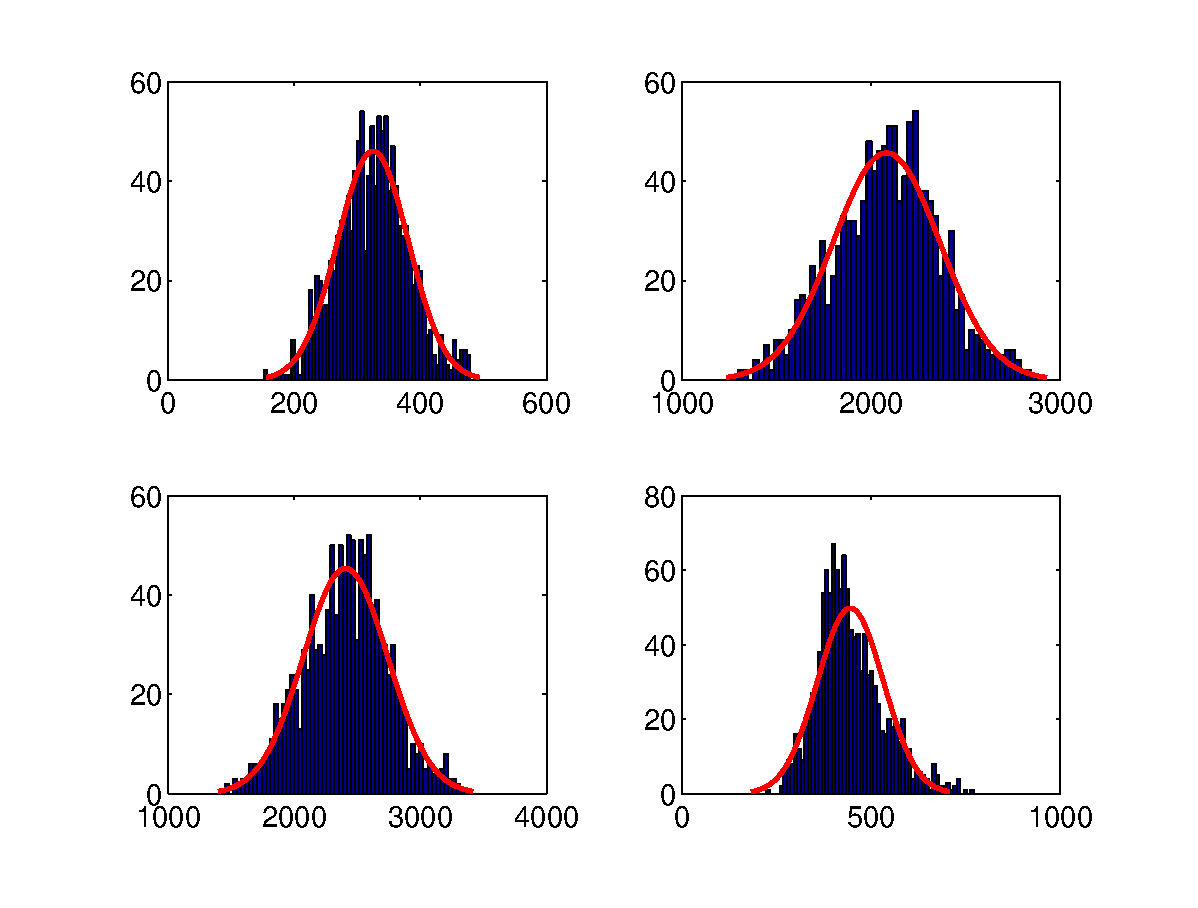
\includegraphics[scale=0.5]{img/histfit_1middleware_push_rop_total_resptime.eps}}
        \caption{The distribution for push throughput (top left), pop throughput (top right), total throughput (bottom left) and response time for 50 SendAndPopSameClient clients using 50 db-connections and 50 worker threads using one (1) middleware.}
        \end{figure}
        
        \begin{figure}[hbtp]
        \centering
        \centerline{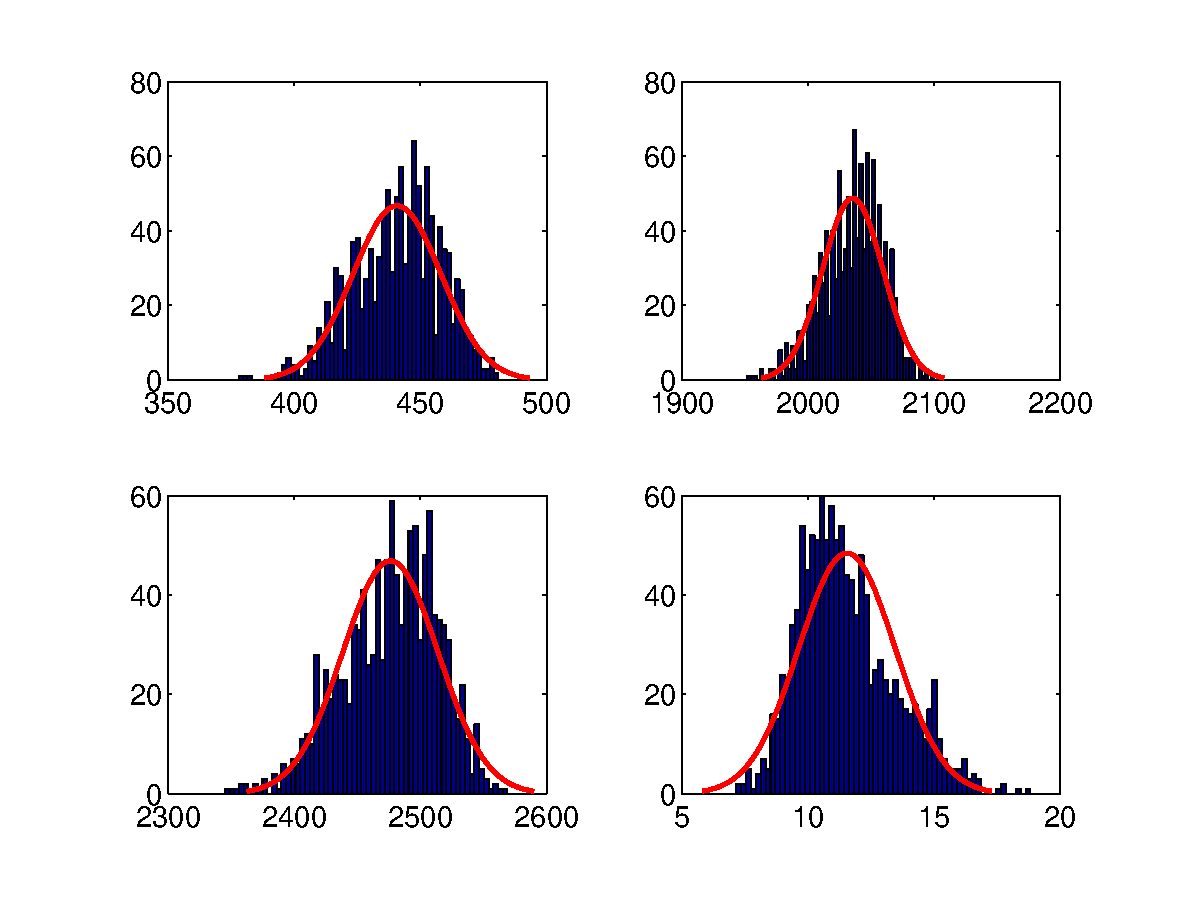
\includegraphics[scale=0.5]{img/histfit_10middleware_push_rop_total_resptime.eps}}
        \caption{The distribution for push throughput (top left), pop throughput (top right), total throughput (bottom left) and response time for 50 SendAndPopSameClient clients using 50 db-connections and 50 worker threads using two (2) middleware.}
        \end{figure}
        
        
        \begin{figure}[hbtp]
        \centering
        \centerline{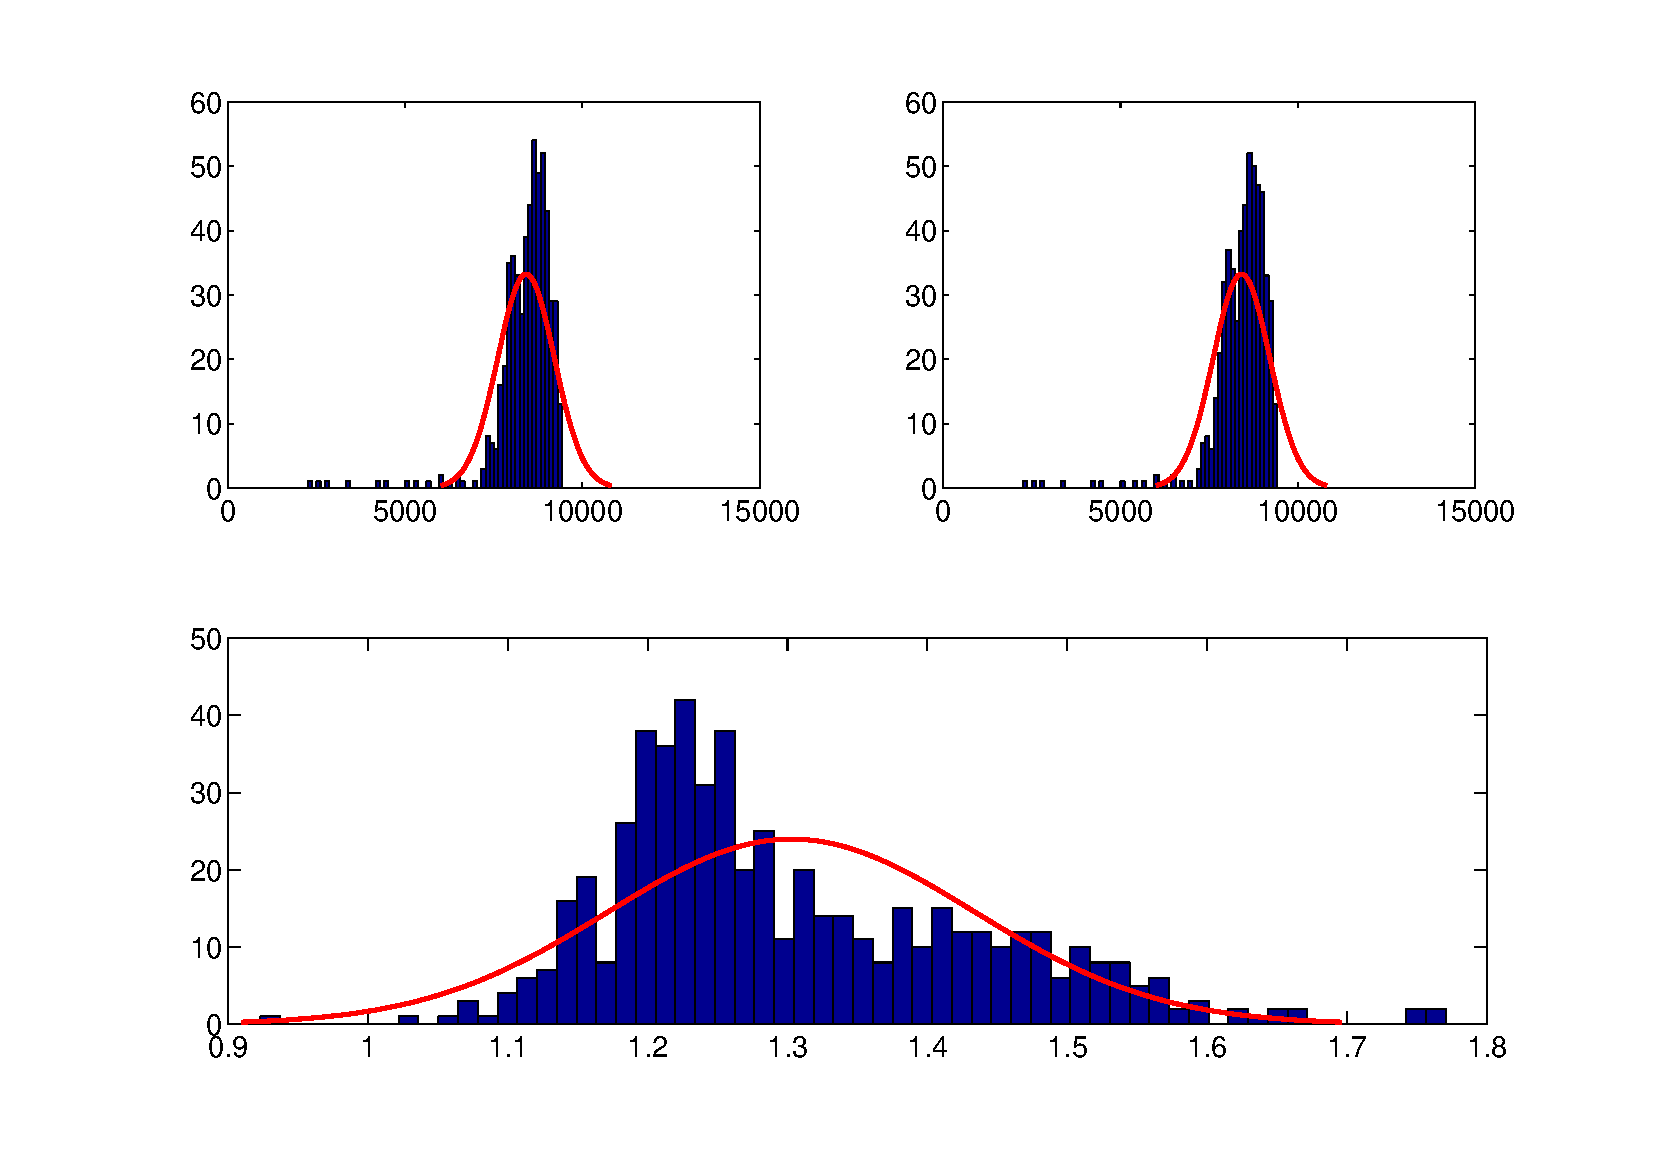
\includegraphics[scale=0.5]{img/histfit_i_fooled_you_50_thrds}}
        \caption{The distribution for push throughput (top left), pop throughput (top right), response time (botto) for 50 SendAndPopSameClient clients and 50 worker threads using one (1) middleware with \textit{I fooled you}-peristence.}
        \end{figure}
        
        \begin{figure}[hbtp]
        \centering
        \centerline{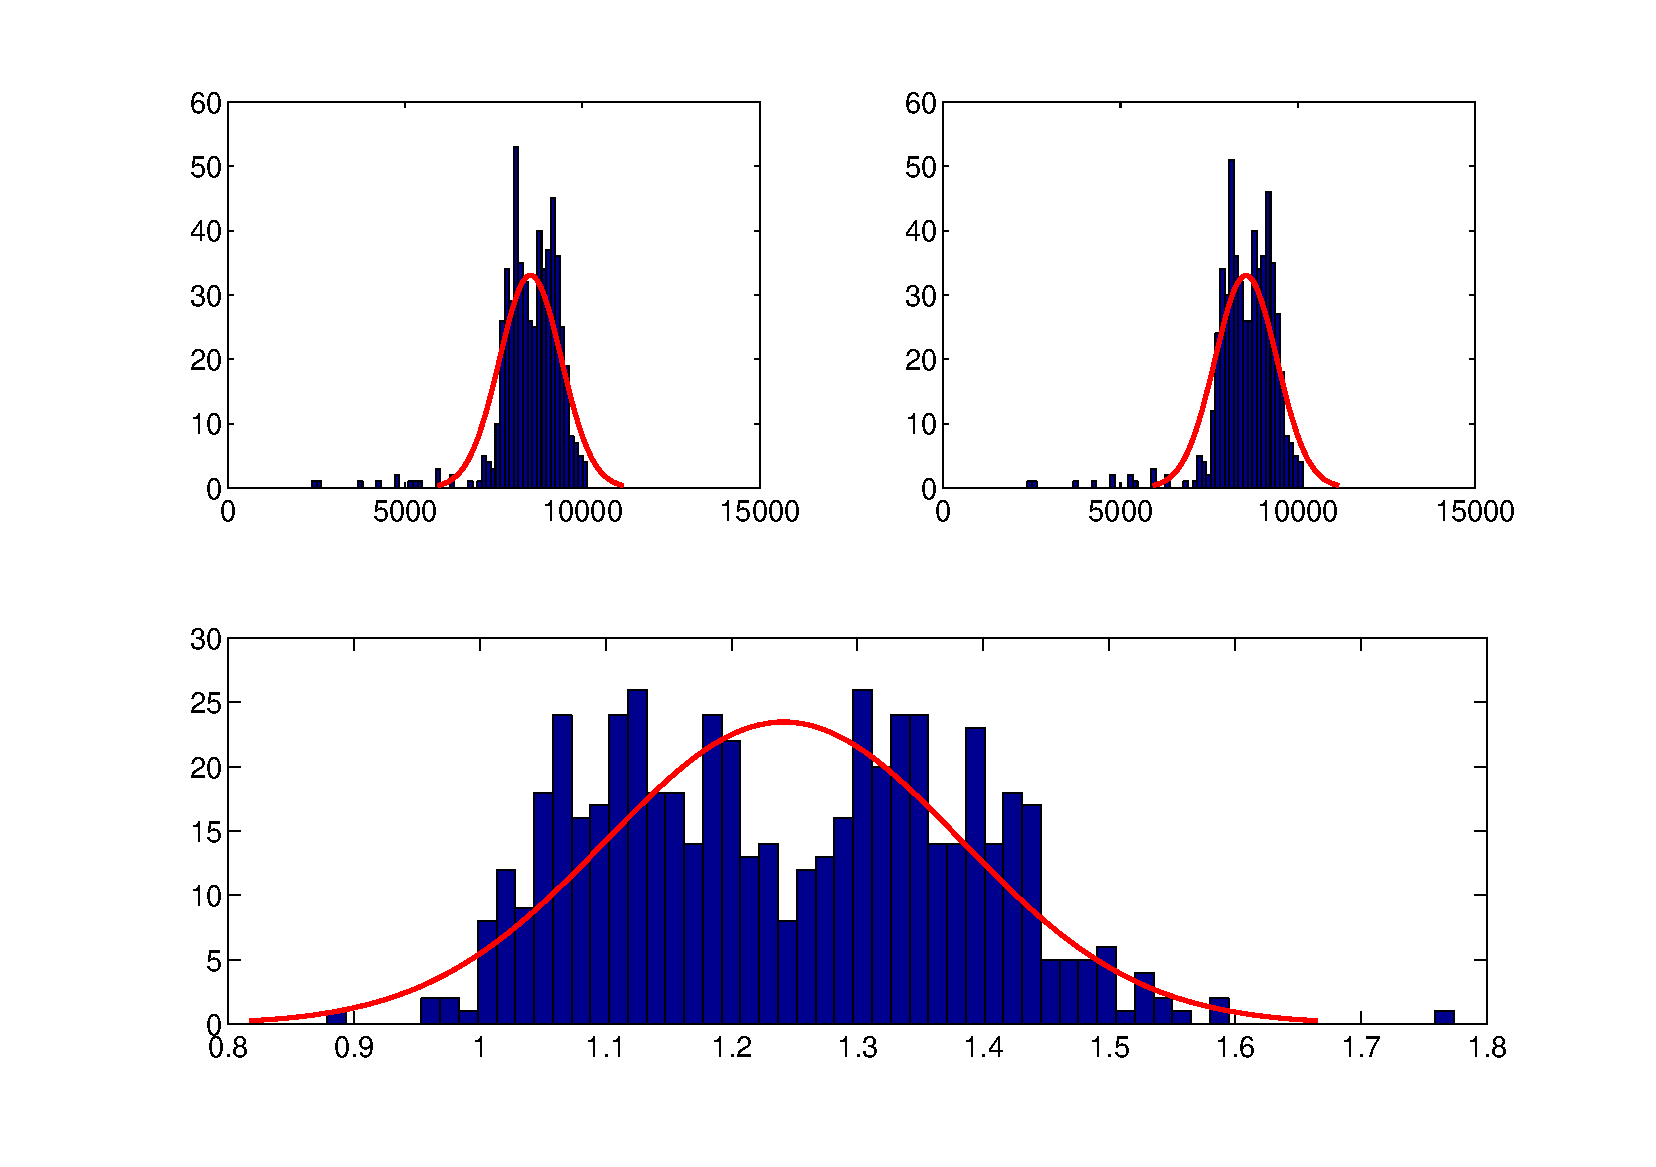
\includegraphics[scale=0.5]{img/histfit_i_fooled_you_5_thrds}}
        \caption{The distribution for push throughput (top left), pop throughput (top right), response time (botto) for 50 SendAndPopSameClient clients and 5 worker threads using one (1) middleware with \textit{I fooled you}-peristence.}
        \end{figure}
        
        
        \begin{figure}[hbtp]
        \centering
        \centerline{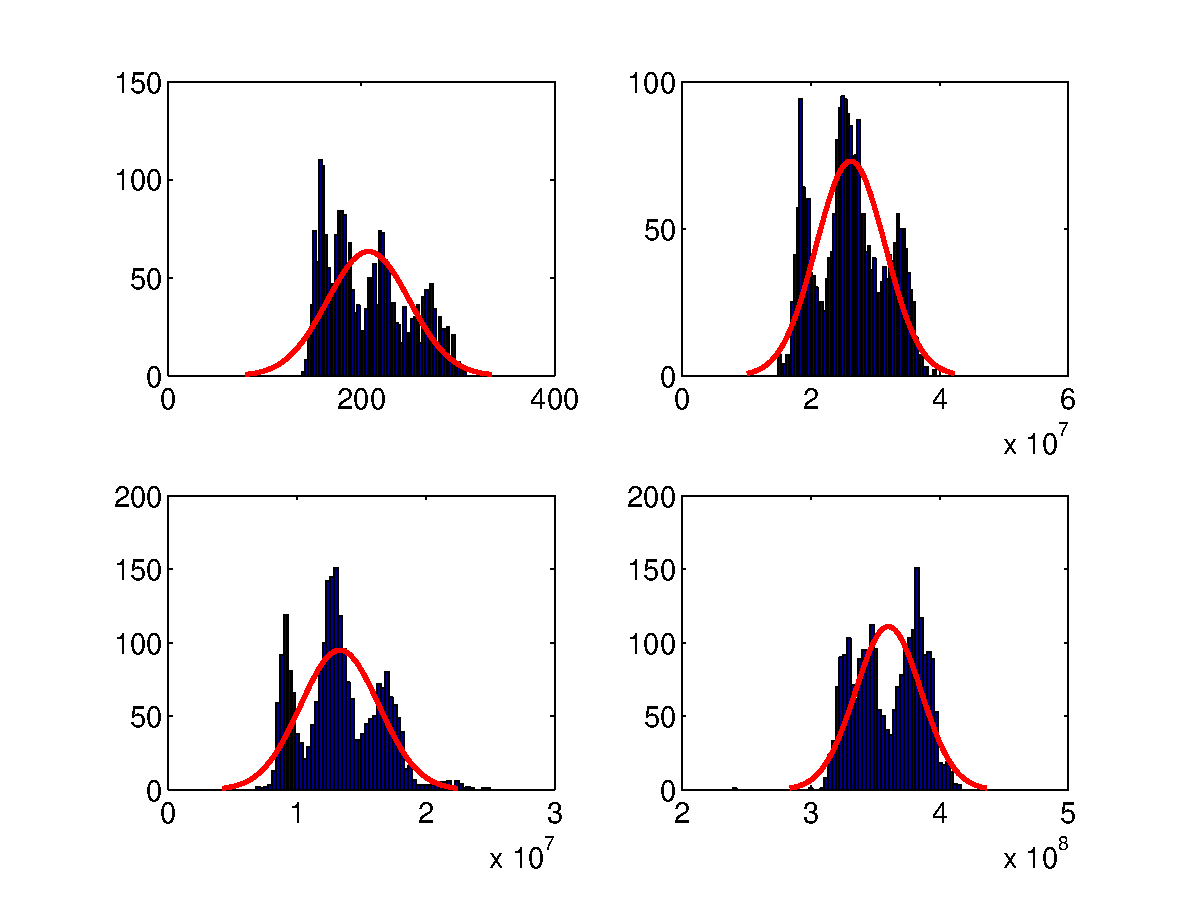
\includegraphics[scale=0.5]{img/histfit_peek_io_crw_db}}
        \caption{The distribution for peek throughput (top left), Socket I/O and Job Creation response time (top right), Client Request Worker response time (bottom left) and Persistence response time (bottom right) for micro benchmarking peek requests.}
        \end{figure}
        
        \begin{figure}[hbtp]
        \centering
        \centerline{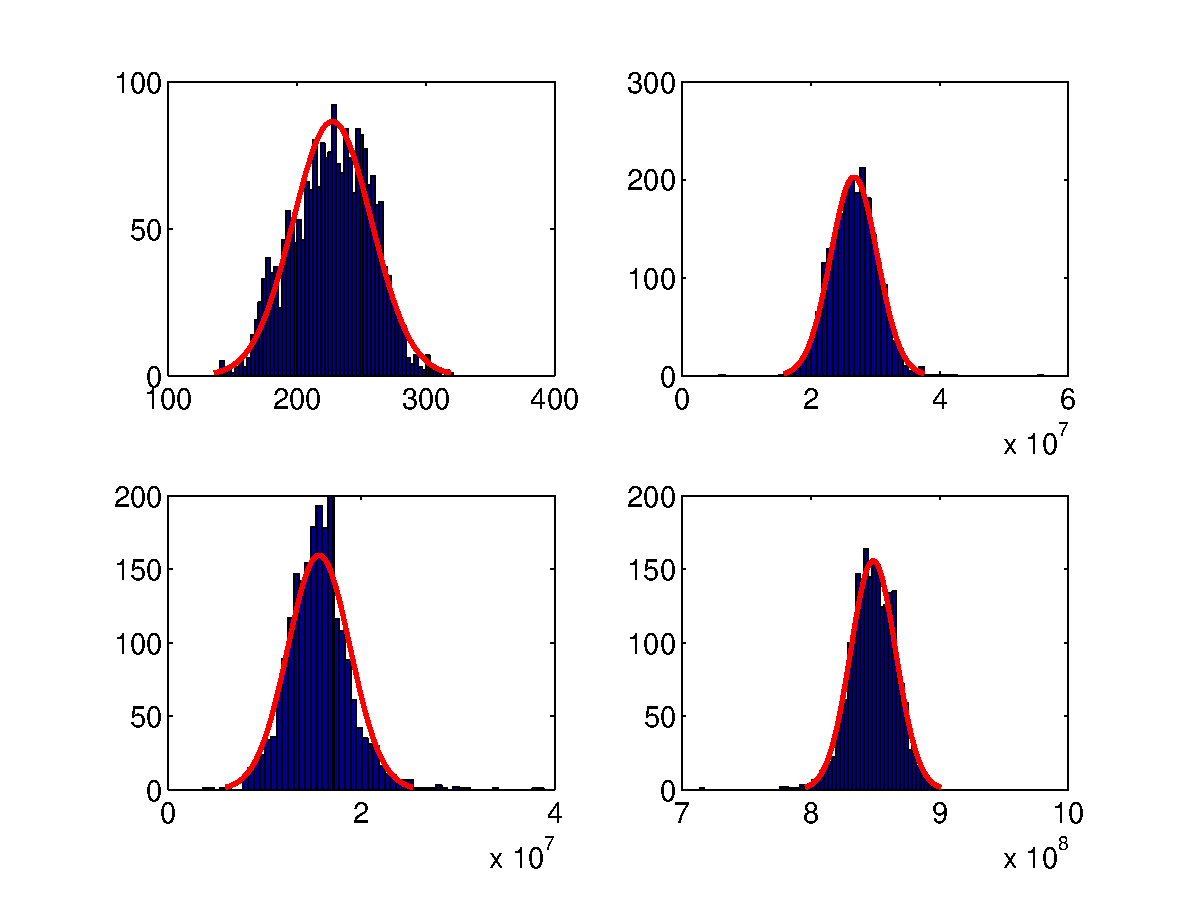
\includegraphics[scale=0.5]{img/histfit_pop_io_crw_db}}
        \caption{The distribution for peek throughput (top left), Socket I/O and Job Creation response time (top right), Client Request Worker response time (bottom left) and Persistence response time (bottom right) for micro benchmarking pop requests.}
        \end{figure}
        
        \begin{figure}[hbtp]
        \centering
        \centerline{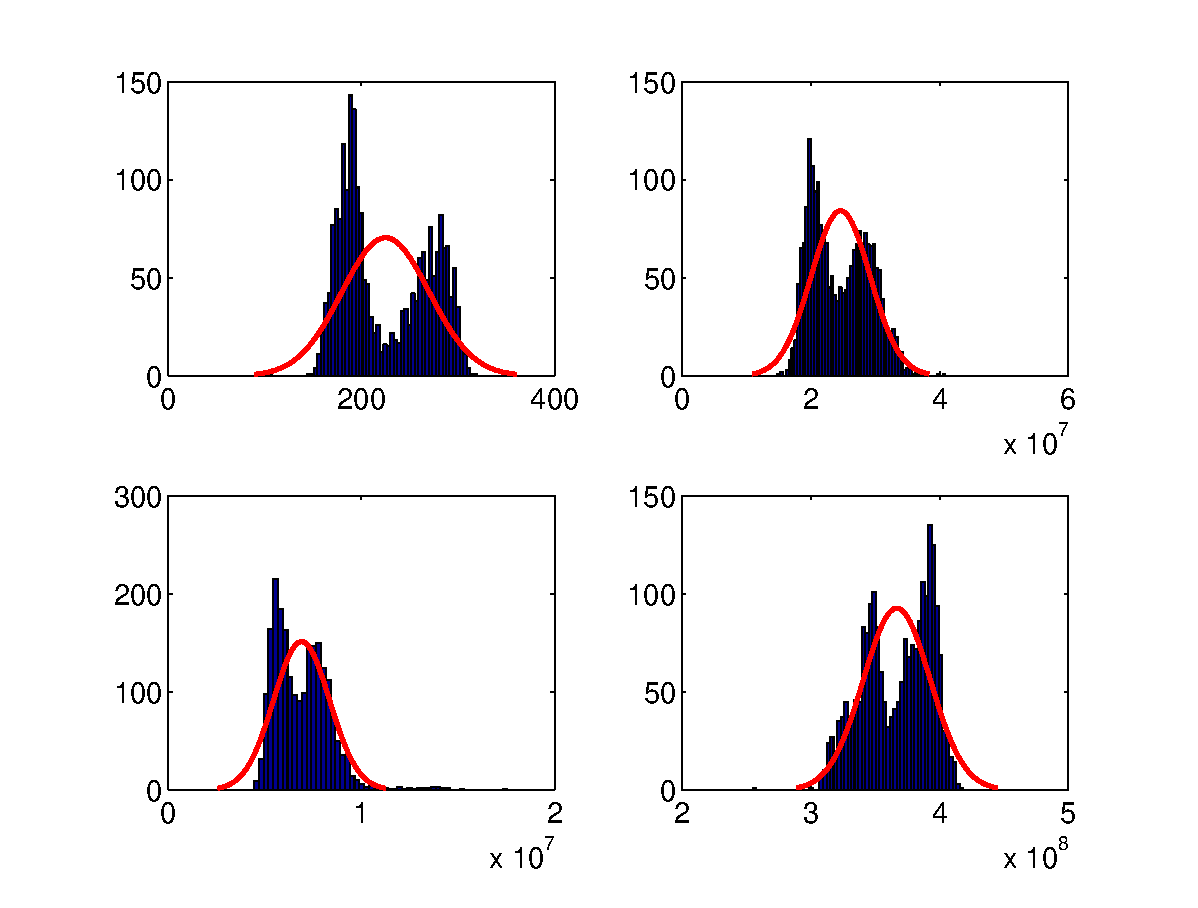
\includegraphics[scale=0.5]{img/histfit_1_push_io_crw_db}}
        \caption{The distribution for peek throughput (top left), Socket I/O and Job Creation response time (top right), Client Request Worker response time (bottom left) and Persistence response time (bottom right) for micro benchmarking peek requests.}
        \end{figure}
        
\end{document}
